\documentclass[11pt, a4paper]{report}
\usepackage[utf8]{inputenc}
\usepackage{amsmath}
\usepackage{amsfonts}
\usepackage{amssymb}
\usepackage{graphicx}
\usepackage{mathtools}
\usepackage[hidelinks]{hyperref}  % most people dont know of this :3
\usepackage[dvipsnames]{xcolor}
\usepackage{systeme}
\usepackage{subcaption}

\usepackage[backend=bibtex,style=verbose-ibid]{biblatex}
\addbibresource{../citations.bib}

\usepackage{listings}
\usepackage{color}
\definecolor{dkgreen}{rgb}{0,0.6,0}
\definecolor{gray}{rgb}{0.5,0.5,0.5}
\definecolor{mauve}{rgb}{0.58,0,0.82}

\lstset{frame=tb,
  language=Python,
  aboveskip=3mm,
  belowskip=3mm,
  showstringspaces=false,
  columns=flexible,
  basicstyle={\small\ttfamily},
  numbers=none,
  numberstyle=\tiny\color{gray},
  keywordstyle=\color{blue},
  commentstyle=\color{dkgreen},
  stringstyle=\color{mauve},
  breaklines=true,
  breakatwhitespace=true,
  tabsize=3
}


\newcommand{\inv}{^{\raisebox{.2em}{$\scriptscriptstyle-1$}}}
\newcommand{\qed}{\hfill $\blacksquare$}

\newcommand{\integers}{\mathbb{Z}}
\newcommand{\rationals}{\mathbb{Q}}
\newcommand{\reals}{\mathbb{R}}
\newcommand{\complexes}{\mathbb{C}}
\newcommand{\field}{\mathbb{F}}

% this makes 'sections' the counted heading, not 'chapters'
\renewcommand{\thesection}{\arabic{section}}

\providecommand{\main}{..} 
\graphicspath{{\main/images/}{images/}}

\author{Jacob Bruner}
\title{IB Extended Essay}
\date{\today}

\begin{document}
\begin{titlepage}
\begin{flushleft}
Dwight School\\
New York, New York
\end{flushleft}

\vspace*{3cm}
\begin{center}
\LARGE Group Theory and Modern Cryptography\\
\vspace*{.5cm}
\large To what extent does group theory provide a mathematical backdrop for modern cryptography? \\
%\vspace*{.5cm}
%\large 340923 words \\
\vspace*{.5cm}
\Large Mathematics \\
\vspace*{.5cm}
\large Full version
\end{center}

\vfill

\begin{flushright}
\begin{tabular}{l@{:\hspace*{\tabcolsep}}l}
Author & Jacob Bruner \\
Advisor & Daniel Bjelis
\end{tabular}
\end{flushright}

\end{titlepage}
\tableofcontents

\pagebreak

\iffalse
############
heres an example of a code block
\begin{lstlisting}
        def intervalValues(z, n):
            return output # return the sequence of values
\end{lstlisting}

heres an example of an image
\begin{figure}[h]
\begin{center}
\includegraphics[scale=.37]{../onefifteen} 
\caption{Sequences Generated by n = 1-15 on Argand Diagram}
\end{center}
\end{figure}
############
\fi


\section{Foreword}

This paper is for research purposes only. Although the information presented is as close to accurate as possible, one should never implement a cryptographic system themselves unless they know \textit{\emph{exactly}} what they're doing. \textbf{I am not liable for any damages caused in testing any cryptographic concepts referenced in this paper.} Cryptography's greatest weakness is human-error, and virtually \textit{all} breaks in cryptographic security result from poor implementation.\autocite{thimbleby}

\section{Introduction and Aim}
\subsection{Topic and Research Question}

For my Extended Essay, I will be exploring the relationship between Group Theory, a mathematical field generalizing symmetry and codifying number systems, and modern cryptography. Cryptography has seen a number of advancements in the computer-age, most notable of which is the use of 'elliptic curves.' In this paper, I intend to show how a group-theoretical perspective on cryptography helps understand elliptic curve cryptosystems. My guiding question is: \textit{to what extent does group theory provide a mathematical backdrop for modern cryptography?}

\subsection{Motivating Idea}
It's undeniable that our modern-day world is reliant on cryptography. Every time a phone sends a text, a browser connects to a server, an email gets sent off, or a monetary transaction is made our devices are performing many hundreds of math operations to ensure our data are 'encrypted.' But what does 'encryption' mean? Let's introduce some definitions. 

‘Encryption’ is the process of disguising a message to be, loosely speaking, hidden to all \textit{except} the intended recipient. This is the process of converting a ‘plaintext’ message into a jumbled ‘ciphertext’, which can be readily shared without risk of the sensitive message leaking. Converting a plaintext message (typically a string/array of characters) into a ciphertext is known as an ‘enciphering’ or ‘encrypting’ transformation. Likewise the reverse operation of recovering the plaintext message from a ciphertext is known as the \textit{deciphering transformation.}\autocite[54]{koblitz} If we denote the plain and cyphertext $\mathcal{P}$ and $\mathcal{C}$ respectively and the enciphering map $f$ and its inverse $f\inv$ we obtain the following diagram:

$$ \mathcal{P} \overset{f}\longrightarrow \mathcal{C} \overset{f\inv}\longrightarrow \mathcal{P} $$

\subsection{The Fundamentals of Symmetric Cryptography}

The intuitive way to implement this cryptosystem has the two transacting parties agree upon the nature of the map $f$ in secret, beforehand. This type of system has a special name, \textit{"Symmetric Key Cryptography"}, reflecting the fact that both parties have the same shared secret. Important historical examples include the 'Caeser Cipher,' where $f$ is a shift operation that maps each letter to a number of places ahead. For instance, the two parties might decide beforehand the map $f$: \textit{shift each character forward 3 letters}, implying the inverse map $f\inv$: \textit{shift each character back 3 letters}. This might look like so: \footnote[0]{One might notice that Ceaser Ciphers are just linear transformations in disguise. Alternatively, we could consider groups of two letters, called \textit{digraphs}, resulting in $f$ being a 2x2 invertible matrix, encoding the shift in a two-by-two matrix. Similarly, we could consider invertible \textit{affine} transformations of the form $f:\vec{x} \to A\vec{x} + \vec{b}$, where A encodes a certain scaling factor.}

\begin{align*}
 \mathcal{P} &\sim A,B,C,D,E,F,...Y,Z  \\ 
 \mathcal{C} &\sim D,E,F,G,H,I,...B,C 
\end{align*} % I'm not sure what symbol to use here...Equivalance relation? Monomorphism?
For example, if one wanted to encrypt the message $\mathcal{P} =$ "HELLO", the ciphertext would be $\mathcal{C} =$ "KHOOR" which they could send off to their friend to decode with the inverse, subtract-three-letters map. Note that, even in this simple example, repeated letters, word length, and other syntactic information provide a lot of information about the nature of the plaintext, making it vulnerable to cryptanalysis techniques.\autocite[56]{koblitz} 

Mathematically, a caeser cipher starts with encoding each letter as a number from $0$, A, to $25$, Z. Of course this depends on what alphabet one uses. We represent this map, shifting $n$ places forward, with addition. Importantly, this operation must 'wrap around' back to zero when it exceeds 'z' in the alphabet. This process, known as \textit{'modular arithmetic'}, is like circling a clock, where after reaching 25 we wrap back to 0. So, in our case, shifting 'z' by 3 letters looks like so: $25 + 3 \bmod 26 \equiv 2$, which reads "25 plus 3 \textit{is congruent to} 2 \textit{modulo} 26." With this in mind, we obtain for each letter $p \in \mathcal{P}$:  

\[
f(p) = p + n \bmod 26 
\]



% I could maybe talk about affine cryptosystems here if I need more words.
% I could also show the linear algebra point of view

Clearly this isn't a very sophisticated cryptographic scheme... For instance, comparing the most commonly occurring letters in the ciphertext to those of the English alphabet could easily break these schemes, broadly referred to as 'substitution ciphers.'\autocite[54]{koblitz} 
Modern techniques are more resistant, where changing one letter of plaintext yields a completely different ciphertext, making modern techniques all but impervious to this technique. 
  
  For instance, AES encryption, part of the modern web standard, is an example of a '\textit{block substitution cypher},' which are beyond the scope of this paper. 
In general, Symmetric-key cryptography (\textit{viz.} predetermined, shared secret) is well understood. For instance, Claude Shannon (\textit{the} father of information theory) proved that the so-called \textit{'one-time-pad'} encryption technique was completely and utterly unbreakable. 
In the general case, he showed that, if a random-generated key is at least as long as the plaintext (specifying a random\footnote{There is a paramount distinction between \textit{random} and \textit{psuedorandom}, the latter of which is vastly easier to implement on a computer. True randomness has to be derived from a non-computer source (for the most part). Commonly implemented approximates include taking the least-significant-digit of a mouse position, or the frequency of keypresses, etc. 
A one-time-pad–like scheme generated from a psuedorandom source \textit{is} breakable, although usually not without some effort.} character for each plaintext character in the same alphabet), then performing a caeser cypher shift on each \textit{individual} plaintext character by the value of the random character, yields a cryptosystem that is \textit{mathematically} impenetrable. 
Or equivalently, performing a random modular addition on each character of the plaintext, with the shared secret being the sequence of random shifts.\autocite{claude} % I maybe should rephrase this in terms of performing a random caeser cipher shift per character if this description is too confusing.
Although modern systems seek smaller key sizes for performance reasons, this worst-case scenario should demonstrate the strength of symmetric-key algorithms in general. The 'one-time-pad' gets its name from its use in WWII when the KGB would distribute palm-sized pads with these one-time-keys and a table to ease in conversion. Such pads were often made of flammable materials to be burned with no trace.\autocite{lewand} 
  
\begin{figure}[h]
\begin{center}
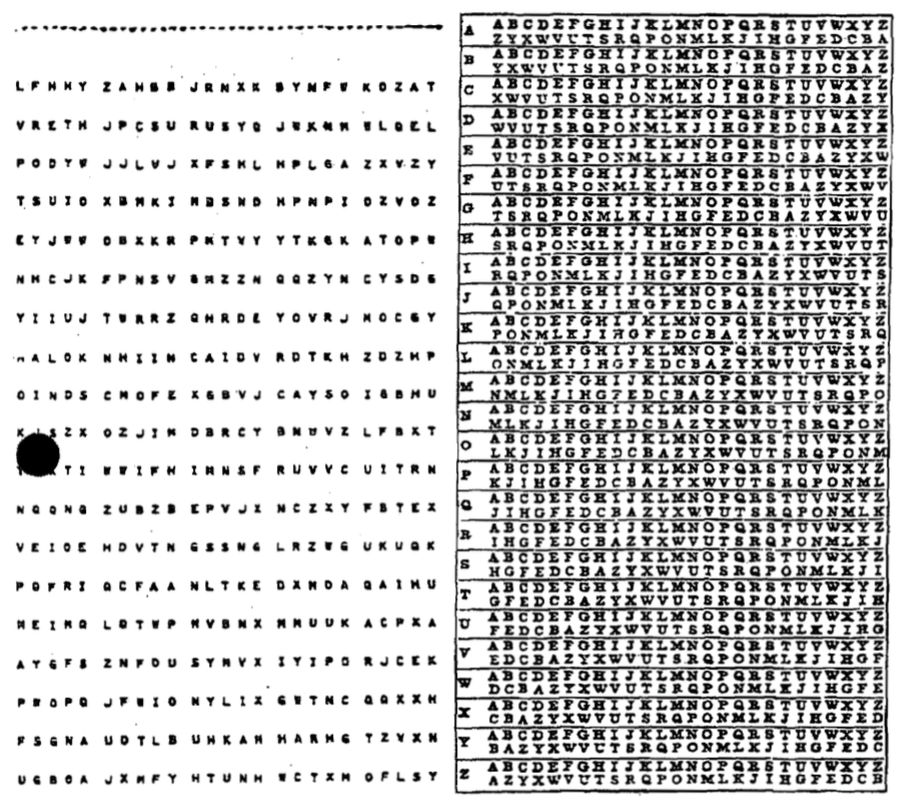
\includegraphics[scale=.29]{diana} 
\caption{Format of a one-time-pad used by the NSA\autocite{diana}}
\end{center}
\end{figure}


\section{What is 'Public-Key' Cryptography}

\subsection{The 'Public-Key' Paradox}

In the modern world, it's impractical to require that every shared secret be determined ahead of time. If a user wants to connect to a twitter server over a secure connection, how could symmetric-key encryption be employed? 
More generally, if two computers want to establish a connection for the first time, is there any way they could do so in an encrypted matter? The intuitive answer might be no, since how could one pass a shared secret without any man-in-the-middle being able to obtain that same key. But this defys the ubiquity of encryption on the internet—every time I connect to a unfamiliar website, I still see a padlock on my browser. How could this be?

%"In applied contexts, the terms "easy" and "hard" are usually interpreted relative to some specific computing entity; typically "cheap enough for the legitimate users" and "prohibitively expensive for any malicious agents"."

\subsection{One-way Operations}

Consider the intuitive fact that some operations are more difficult to do forwards than in reverse—certain 'one-way functions.' For instance, if I mixed two different-colored paints together and asked whether you, \textit{a priori}, could deduce the two initial colors given the end result, would you be able to? Although its quite easy to check whether any two colors combine to match the end result, there isn't an \textit{easy} operation that takes the end result returning the initial colors. This happens to be true in mathematical contexts as well. 

The foremost 'one-way operation,' employed to this day, is that of multiplying large numbers with minimal divisors. This makes sense from a practical standpoint; breaking up a large number into its factors usually boils down to computationally expensive trial divisions, to use a jargon, its \textit{asymptotic time-complexity is exponential}, meaning that the time required to reach an answer scales exponentially with the size of the number. Algorithms like the general-number-field-sieve quicken this slightly,\autocite[1482]{pomerance} but regardless it is vastly faster to compute multiplication, the time complexity of which scales \textit{at worst} with the square of the number.\autocite{bunimov}

\subsection{Diffie-Hellman Key Exchange}

The Diffie-Hellman protocol was the first asymmetric protocol,\footnote{Although this isn't a true "public-key" algorithm, rather its a non-authenticated key exchange, DH can be easily modified to send arbitrary messages in a scheme known as 'Elgamal encryption,' which is true "public-key" cryptography.\\\autocite{elgamal}} using the above intuition as a starting point. The end result of the key exchange is a commonly shared number, which can then function as the key for them to establish symmetric encryption.

Between two parties, Alice $A$ and Bob $B$, the protocol first agrees on a common 'generator' integer $g$, and this can be done over an eavesdropped channel. Each party chooses another \textit{secret} integer in private: their private key. Say, Alice chooses $a$ and Bob chooses $b$. Then, each party exponentiates the generator by their private key. So Alice and Bob compute $g^a$ and $g^b$ respectively. Each then sends this result to the other over the insecure channel. Finally, they both exponentiate the received numbers by their private key. For example, Alice would receive $g^b$ over the network, then compute$(g^b)^a$.
By the commutativity of integer multiplication, multiplying $g$ by itself $b$ times \textit{then} $a$ times is the same as  multiplying $g$ by itself $a$ times \textit{then} $b$ times. Explicitly, with Alice and Bob's private-keys in \color{orange}{amber} \color{black}{and} \color{blue}{blue} \color{black}{respectively:}
\[ (g^{\color{orange}{a}}\color{black}{)}^{\color{blue}{b}} = g^{\color{orange}{a}\color{blue}{b}} = (g^{\color{blue}{b}}\color{black}{)}^{\color{orange}{a}}  \]

\begin{figure}[ht]
\begin{center}
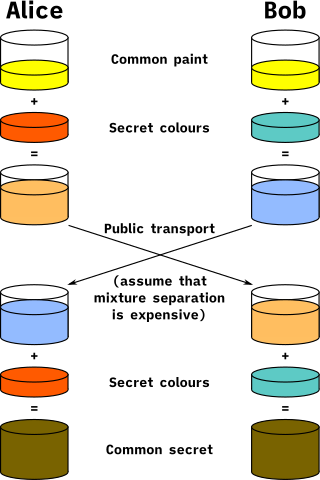
\includegraphics[width = .4\linewidth]{colors} 
\caption{Diffie-Hellman protocol depicted visually, with mixing and separating paint replacing multiplication and factorization. (public domain)}
\end{center}
\end{figure}

The one caveat to the above description, however, is that these multiplications are performed \textit{modulo} $n$ for some integer $n$. As discussed before, this means numbers wrap around 'like a clock'; if $g^a$ exceeds $n$, the remainder of $g^a \div n$ is returned. This should make sense, because computers have limited memory and because exponentiation by a (large) number yields a incomprehensibly large result—too large to send over a network or perform computation with. Additionally, computers can perform modular exponentiation \textit{very} performantly by leveraging tricks in binary.\autocite{bunimov}

Our relation from before looks like:
\[ (g^{\color{orange}{a}}\color{black}{\:\mathrm{mod}\; p)}^{\color{blue}{b}}\color{black}{\:\mathrm{mod}\; =\; }g^{\color{orange}{a}\color{blue}{b}} \:\mathrm{mod}\; p = (g^{\color{blue}{b}}\color{black}{\:\mathrm{mod}\; p)}^{\color{orange}{a}} \color{black}{\:\mathrm{mod}\; p.}  \]
Importantly, though, Alice and Bob both agree on a common result $g^{ab}\;\mathrm{mod}\;p$.

In the real world, this type of Diffie-Hellman transaction is used by countless devices every second to allow secure connections over the internet. Browsers have a predetermined set of generators from the National Institute of Standards and Technology (NIST) which they use to establish a shared secret with a web-server which is then used to implement symmetric encryption to facilitate fast data transfer. Every time you are to connect to a \texttt{https://}... website, with the padlock in the corner, the client (you) and the server are performing this type of key exchange. Although, modern implementations might use a different 'number system' to perform the repeated multiplications...
% wow i didn't know \bmod was a thing.... :P

\subsection{A Proof that: $(a \bmod p)^k \bmod p = a^k \bmod p$}

Here I offer a short proof verifying the ideas above.
Given the linearity of modularity over multiplication:
$$a \times b \bmod n = (a \bmod n) \times (b \bmod n) \bmod n$$
I will show that $(a \bmod p)^k \bmod p = a^k \bmod p$ with induction.
\vspace*{0.4cm}

\textbf{Basis} case, $P(1)$ or $k=1$, holds since,

\[ a^1 \bmod p = (a \bmod p)^1 \bmod p \tag{basis}  \]

\textbf{Assume} $P(k)$ holds for all $k$ like so:

\[ a^k \bmod p = (a \bmod p)^k \bmod p \tag{P(k)} \]

Now, multiplying $ \bmod p$ both sides by $(a \bmod p)$ and applying the given:
\begin{align*}
a^k \bmod p \times a \bmod p \mod p &= (a \bmod p)^k \bmod p \times a \bmod p \mod p\\
(a^k \times a) \bmod p  &= ((a \bmod p)^k (a \bmod p)) \bmod p\\
a^{k+1} \bmod p  &= (a \bmod p)^{k+1} \bmod p \tag{P(k+1)}
\end{align*}

Hence, since $P(1)$ holds and $P(k) \Rightarrow P(k+1)$, the proposition holds for all positive integers.
\qed


\section{An Introduction to Group Theory}
Transitioning from the methods described earlier, I will now explore how many of these concepts fit into a group-theoretical perspective and how these tools can illuminate a path to inventing stronger cryptosystems.

\subsection{The Group Axioms}

  A group is a set $G$, equipped with a binary operation mapping two elements to another of the form $\ast:\ G \ast G \to G$ such that the following conditions hold:\autocite[16]{saracino} \linebreak
\\\textbf{Associativity}
\\$\text{For all } a,b,c \in G,\ a\ast(b \ast c) = (a\ast b) \ast c$
\\\textbf{Identity}
\\$\text{There exists an } e \in G \text{ such that } a \ast e = e \ast a = a \ \text{ for all } a \in G$
\\\textbf{Inverse}
\\$\text{Each } x \in G \text{ has an inverse } x\inv \in G \text{ with } x \ast x\inv = x\inv \ast x = e \hspace*{.5cm}\footnote{Note that uniqueness of inverses is not given in the axioms for a group, since it follows from the Identity and Associativity requirement and the existence of a (not strictly unique) inverse. If $b, c$ are left and right inverses respectivly of an element $a$ with identity $1$, then considering $c = 1 \ast c = (b \ast a) \ast c = b \ast (a \ast c) = b \ast 1 = b$, gives us $b = c$ as required.}$
\linebreak

Under this axiomatic definition of a group, a few canonical examples might come to mind.
 
 For instance, the integers form a group under addition $(\mathbb{Z}, +)$. It's worth verifying for yourself that these do fit the definition of a group. Our identity element is 0, since $0 + a = a + 0 = a$ for all $a \in \mathbb{Z}$. Addition of integers is clearly associative. And, every number has a unique inverse, $a\inv := -a$. 
 
 Similarly, the real numbers (excluding 0) might form a group under multiplication, write $(\reals\setminus\lbrace 0 \rbrace, \times)$ or $\reals^{\times}\setminus\lbrace 0 \rbrace$. 
We verify it has a two-sided identity, $1$; that its operation is associative; and that every element has an inverse $a\inv := \frac{1}{a}$, since $a\times \frac{1}{a} = \frac{1}{a} \times a = 1, \ \forall  a \in  (\reals\setminus\lbrace 0 \rbrace, \times)$. 
 
 To help intuition,consider that the integers $(\mathbb{Z},\times)$  \textit{do not} form a group under multiplication, since inverses are not suitably defined, i.e., there is no integer $a$ such that $a\times 2 = 2 \times a = 1$.

\subsection{The Case for Commutativity and Abelian Groups}
One key property that we didn't require in our group axioms is \textit{commutativity}. At first glance, this might seem like an obvious condition, since many of the introductory examples do obey commutativity. But most of the insight that comes from group theory is from the study of non-commutativity. This distinction happens to be so important that commutative groups have a special name: \textit{abelian groups}.\autocite[17]{dummit} Likewise, groups that violate this condition are sometimes called \textit{non-abelian groups}. In general, non-abelian groups can be thought of as corresponding to symmetries that change the backdrop for another symmetry to occur. For instance, the group of symmetries on a square, $\mathrm{D}_{8}$, is non-abelian (meaning non-commutative). If you labeled the verticies of a square, you'd find performing a rotation and than a reflection is not, in general, the same as performing a reflection than a rotation\footnote[0]{If we were working with the presentation of $\mathrm{D}_8$, $\langle a,x\ \vert \ a^4 = x^2 = e,\ xax\inv = a\inv \rangle$, we would say that $x$ and $a$ don't commute—corresponding to the reflection and rotation generators respectively.}. Despite this, many of the examples we have and will look at happen to be abelian. For instance, the additive and multiplicative (sans $0$) groups of $\integers, \rationals, \reals$ and $\complexes$, are  'abelian.' To highlight the importance of commutativity, consider that many properties of electric charge, as described by the Standard Model (in Quantum Field Theory), follow directly from the commutativity of the circle group $U(1)$ or $T$.\autocite{weinberg} But this is far beyond the scope of basic group theory.

\subsection{Applying Group Theory to Cryptography: Cyclic Groups}

  Much of the groups that are of importance to cryptography are abelian groups. For intuition on why this may be the case, consider the Diffie-Hellman example before. Both parties combined a series of steps involving their generator and private keys. If the underlying multiplicative group were not abelian, $(g^a)^b$ doesn't necessarily equal $(g^b)^a$. Similarly, in the case of a one-time-pad, if our modular addition weren't commutative, our results would be unpredictable. This provokes the question, were these cases abelian groups?
 
 The group of integers under addition \textit{modulo} $n$ is denoted $(\integers / n \integers, +)$ or just $\integers / n \integers$  and is called the 'cyclic group of order $n$.' In an earlier example, we performed operations in $(\integers / 26 \integers, +)$ so as to not surpass the alphabet. The notation here is actually meaningful. Without delving too far into 'quotient groups' and 'normal subgroups,' the slash corresponds to 'quotienting' out the integers by $p$ times the integers, creating a group where $1$ is indistinguishable from $p+1$ and indeed $2p+1, 3p+1, -p+1, -2p+1...$, called an \textit{equivalence relation}.\autocite[104]{saracino} This formalizes the impercise notions of 'going around a clock face.'
  
  Contrastingly, performing multiplication in a modular fashion forms the group $(\integers / n \integers, \times)$ or $(\integers / n \integers)^{\times})$. This group behaves a little differently and consists of the elements $\lbrace 0, 1 ...,n-1\rbrace$ that are relatively prime to $n$, i.e., share no nontrivial divisors. In this multiplicative group, it takes more care to define inverses than in the more familiar examples. Inverses can be computed using the Euclidean Algorithm or by leveraging the symmetries in modular multiplication. Essentially, in $(\integers / n \integers)^{\times})$, the multiplicative inverse of a number $n$ is a number $m$ such that,
\[ nm \equiv 1 \mod p\]

Now, proving that the elements are only those relatively prime to $n$, consider that the invertible elements of $(\integers / n \integers)^{\times})$ (for any $q$) are exactly those that are relatively prime to $q$. The proof is by contradiction:

	If $\mathrm{gcd}(n,q) = d$ (i.e., they share a nontrivial divisor) with $d \neq 1$, assume there is some $m$ for which $nm \equiv 1 \mod p$. Expanding this out,
\begin{align*}
	nm &\equiv 1 \mod p\\
	nm - 1 &\equiv 0 \mod p\\
	\Rightarrow &\hspace*{0.3cm} p | nm-1\\
	\Rightarrow &\hspace*{0.3cm} d | nm-1\\
	\Rightarrow &\hspace*{0.3cm} d | nm-1 -nm\; (\text{since } d|nm)\\
	\Rightarrow &\hspace*{0.3cm} d | 1
\end{align*}
As $1$ is not divisible by anything except $1$, our assumption was false and $n$ cannot have an inverse and is not $\in (\integers / n \integers)^{\times})$.\autocite[19]{koblitz} 
\qed

Notice that for prime $p$, every number $< p$ is relatively prime to $p$, so the order of the group $(\integers / n \integers)^{\times}$ is $p-1$, which you might notice is the same as the order of $(\integers / n \integers)^{+}$. This fact will be useful in a bit.


\subsection{Discrete Logarithm Problem}

In this section, I want to explore the formal statement of 'why' certian operations are difficult to reverse, although  In a Diffie-Hellman key exchange over $(\integers / q \integers)^{\times}$, Alice and Bob were using the map $f$,
\[ f(n) = g^n \bmod q \]
or, written in terms of their respective groups,
\[ f: \integers \rightarrow (\integers / q \integers)^{\times} \]
This $f$ is a function between groups (a \textit{group homomorphism}) from $\integers$ \textit{onto} a \textit{\textbf{subset}} of $(\integers / q \integers)^{\times}$ surjectively, namely the subset generated by $g^n$ which I will denote $H$. The inverse mapping here (the 'computationally difficult' part), isn't defined for the entirety of $\mathrm{dom}\: f$, since $f$ takes an infinite group $\integers$ to a subset $H$ of the finite group $(\integers / q \integers)^{\times}$. 

Roughly sketching the 'why' behind what is to follow, it can be shown that any finite abelian group must consist of cyclic groups as building blocks, cyclic groups being the integers under addition modulo some $n$. \footnote{By the (aptly named) Fundamental Theorem of Finitely Generated Abelian Groups. \\\autocite[134]{saracino}} Hence, our subset $H$ (which one can prove forms a group as well, a 'subgroup') must be one of these cyclic groups. We can then write this sort-of inverse map $f\inv$ as,

\[ \log_g : H \rightarrow (\integers / m \integers, +) \]

Ascertaining this 'hidden' cyclic subgroup $H$ is known to be a difficult problem, and this difficulty of computing the original integer $n$ is infeasible since $\log_g$ does not map back to all the integers: just some additive group of the integers modulo some $m$. This is known as the \textit{discrete logarithm problem}.\autocite[97]{koblitz} Like discussed before with division, there is no known algorithm that can solve a discrete logarithm with time-complexity that scales polynomially (on a non-quantum computer). It remains an open question in theoretical computer-science whether such a polynomial-time algorithm exists, though all of  modern cryptography rests on this principle.


\section{Group Law on an Elliptic Curve}
\subsection{Definition of an Elliptic Curve}
In a complete turn of events (that will hopefully make sense in the end), I want to explain the notion of \textit{Elliptic Curves}. Elliptic curves are a family of  algebraic\footnote{Specifically a dimension one algebraic variety since it admits a group structure.} curves defined as the solution set of a polynomial equation. Namely, an elliptic curve is the set of solutions $(x,y)$ to an equation of the form:\autocite[10]{koblitz} \footnote{The general form of an elliptic curve $y^3 + a_1xy + a_2y = x^3 + a_3x^2 + a_4x + a_5$ can always be transformed in a series of scalings and rotations to the reduced form preserving the group structure as long as the field is of characteristic not 2 or 3.}
\[y^2 = x^3 + ax + b, \text{ for constants } a,b.\]
Importantly, the behavior of this curve is dependent on the ground 'field' on which one defines it. We will look at the familiar case of the reals shortly, but this is an important distinction, hinting towards the possibility of a discrete context, or field, to come. Field, in mathematics, refers to a structure where any two elements have a well-defined notion of addition, subtraction, multiplication and division (except by a 0 element). The most important examples are the rationals $\rationals$, the reals $\reals$, and the complex numbers $\complexes$. Not the integers since, take, for example: $1, 2 \in \integers$, but $\frac{1}{2} \notin \integers$. We will begin with the case of an elliptic curve over the reals.

\subsection{Elliptic Curves over the Reals}

\begin{figure}[h]
\begin{center}
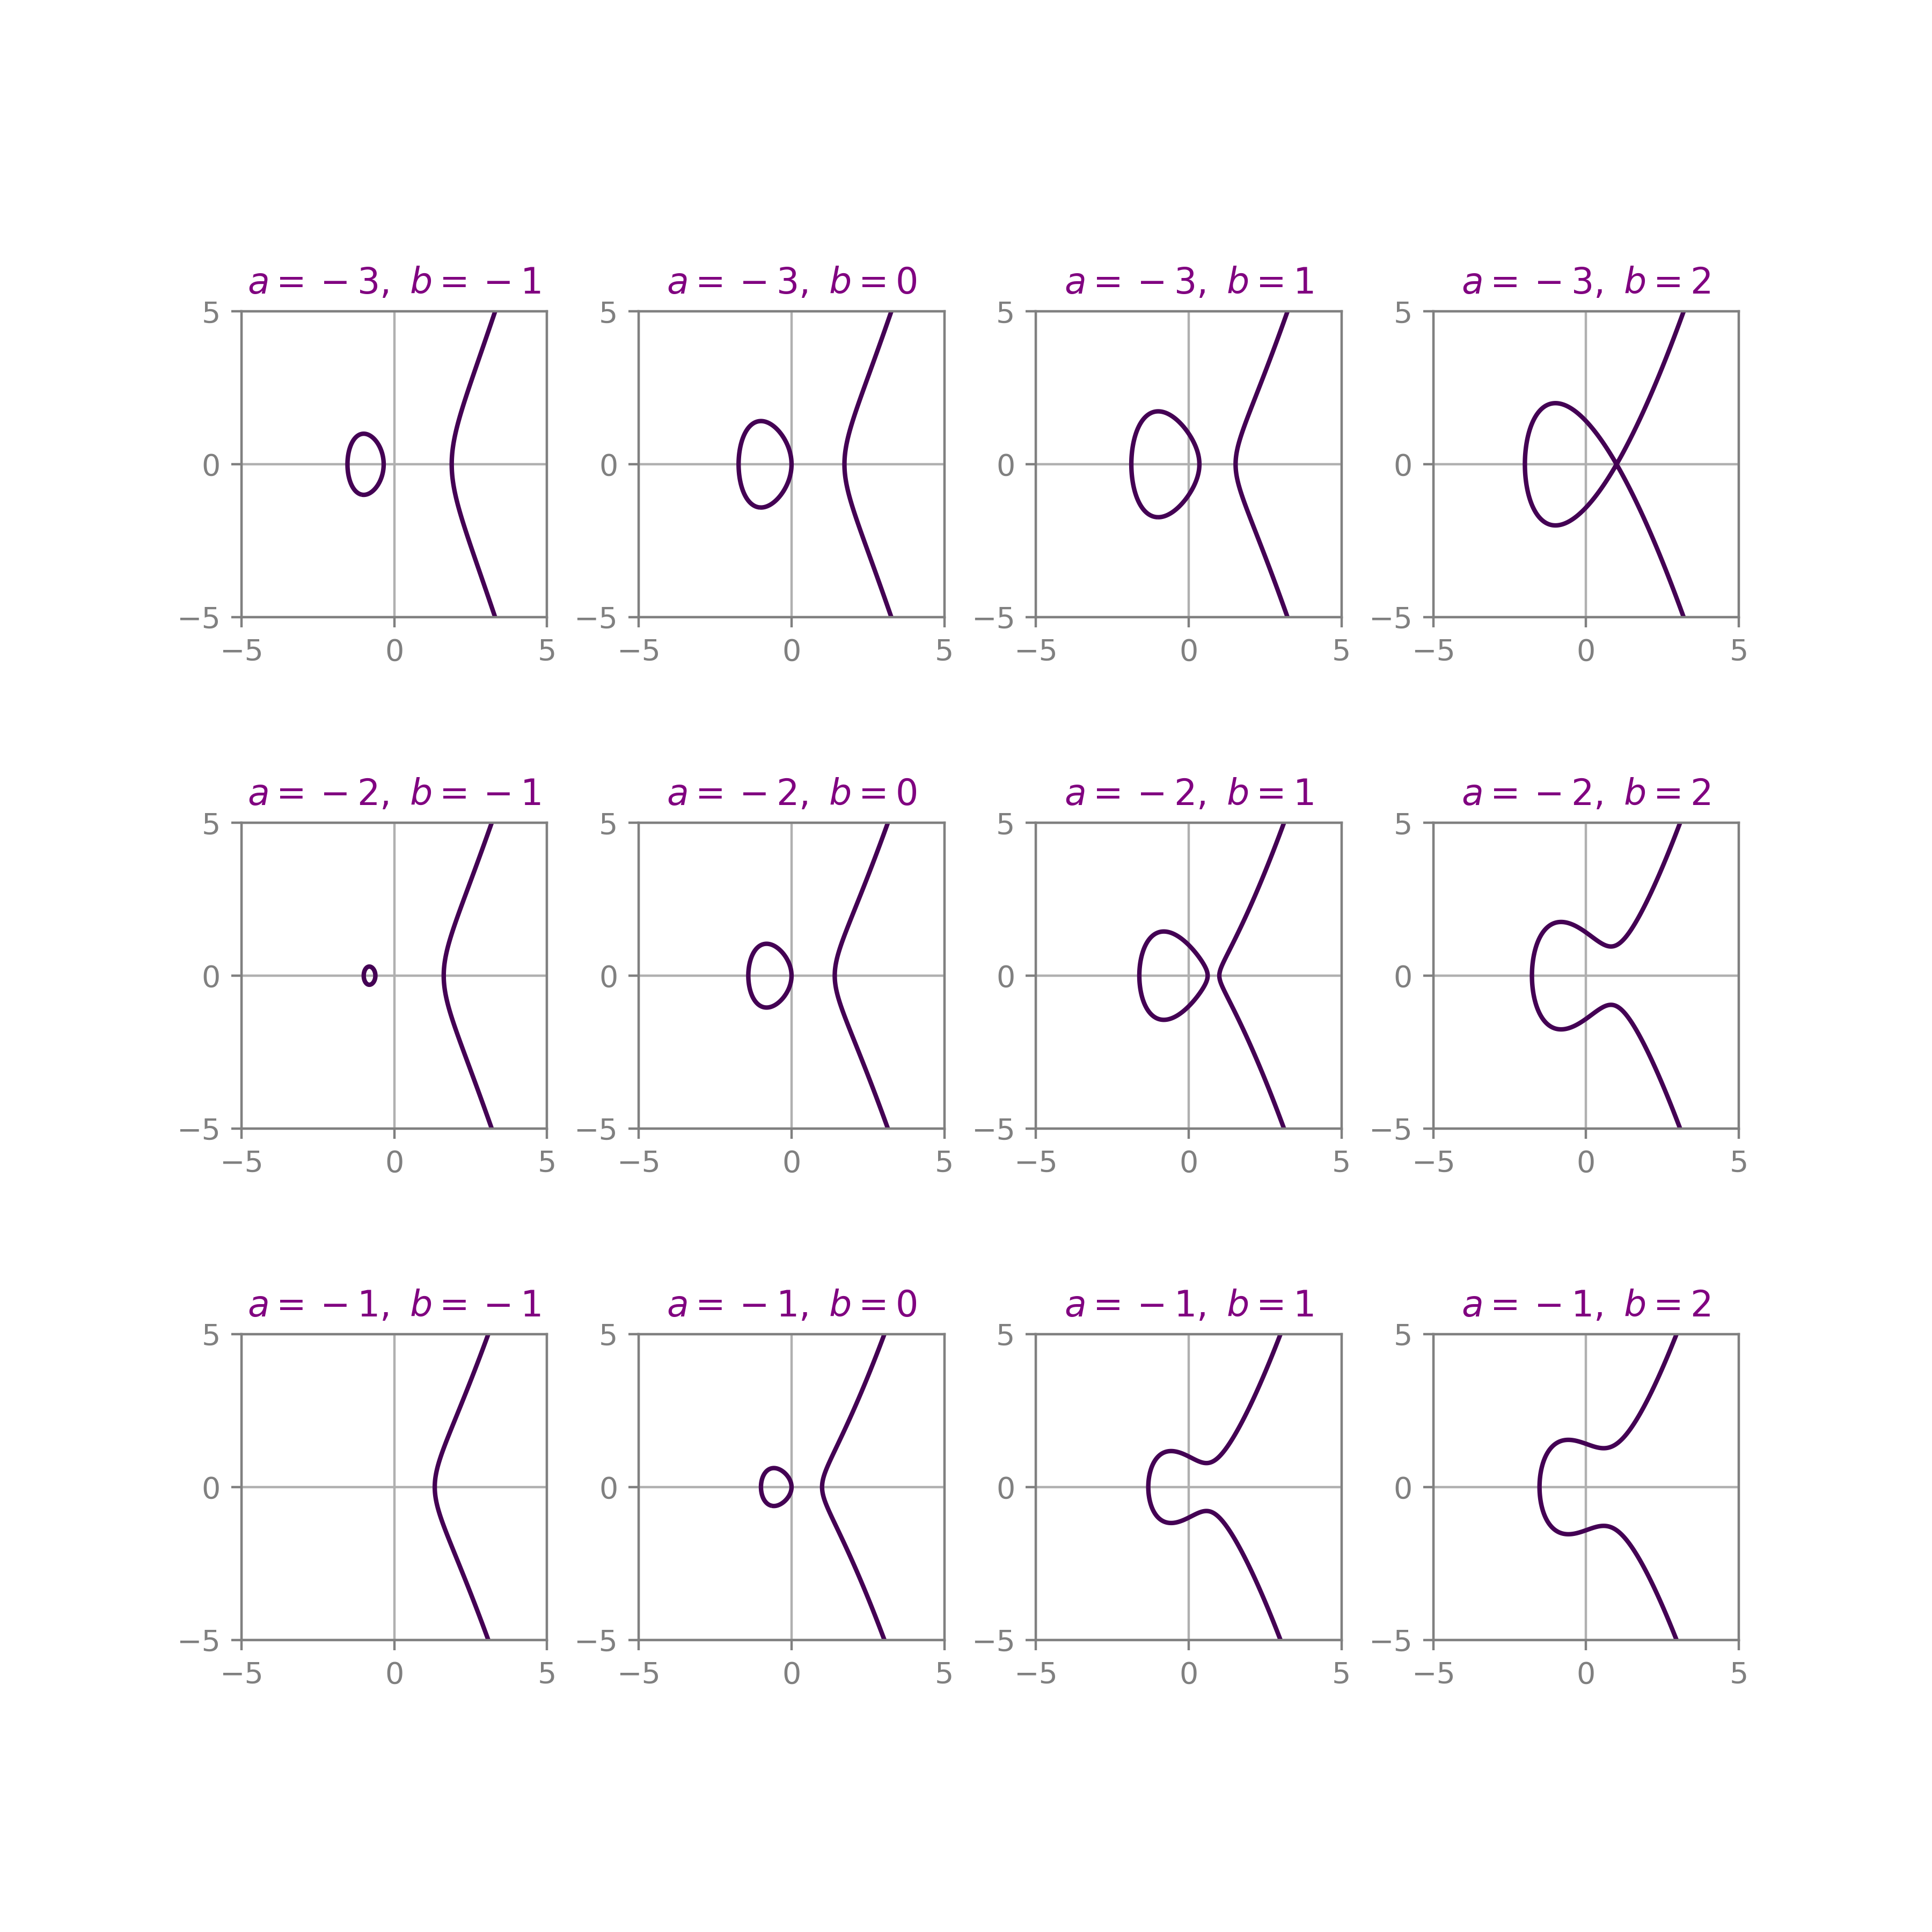
\includegraphics[width=\linewidth]{elliptic_curves.png} 
\caption{A few selected elliptic curves plotted with matplotlib over the reals with $a$ from $-3$ to $0$ and $b$ from  $-1$ to $2$.}
\label{fig:realECs}
\end{center}
\end{figure}

In \ref{fig:realECs}, we see the general shape of an elliptic curve, usually with a sort-of bulbous head on the left. This complicated shape arises from square rooting a general depressed cubic of the form $y=x^3+px+q$. Without the $x^2$ term, this cubic is guaranteed to have only one inflection point at $x=0$, since its second derivative $y'' = 6x$ does not depend on $p$ or $q$. Since square roots preserve the inflection points, we  can see the connected graphs in \ref{fig:realECs} all have inflections at zero.
Furthermore, the process of square-rooting increases values from $0<y<1$ and decreases values when $y>1$ with a fixed point at $1$. Over $\reals$, square roots are limited to inputs greater than $0$, but since we take both branches $(\pm)$ of the root, we see reflection symmetry across the y-axis (this will be important in a moment). To illustrate the relationship: 
\begin{figure}[ht]
\begin{center}
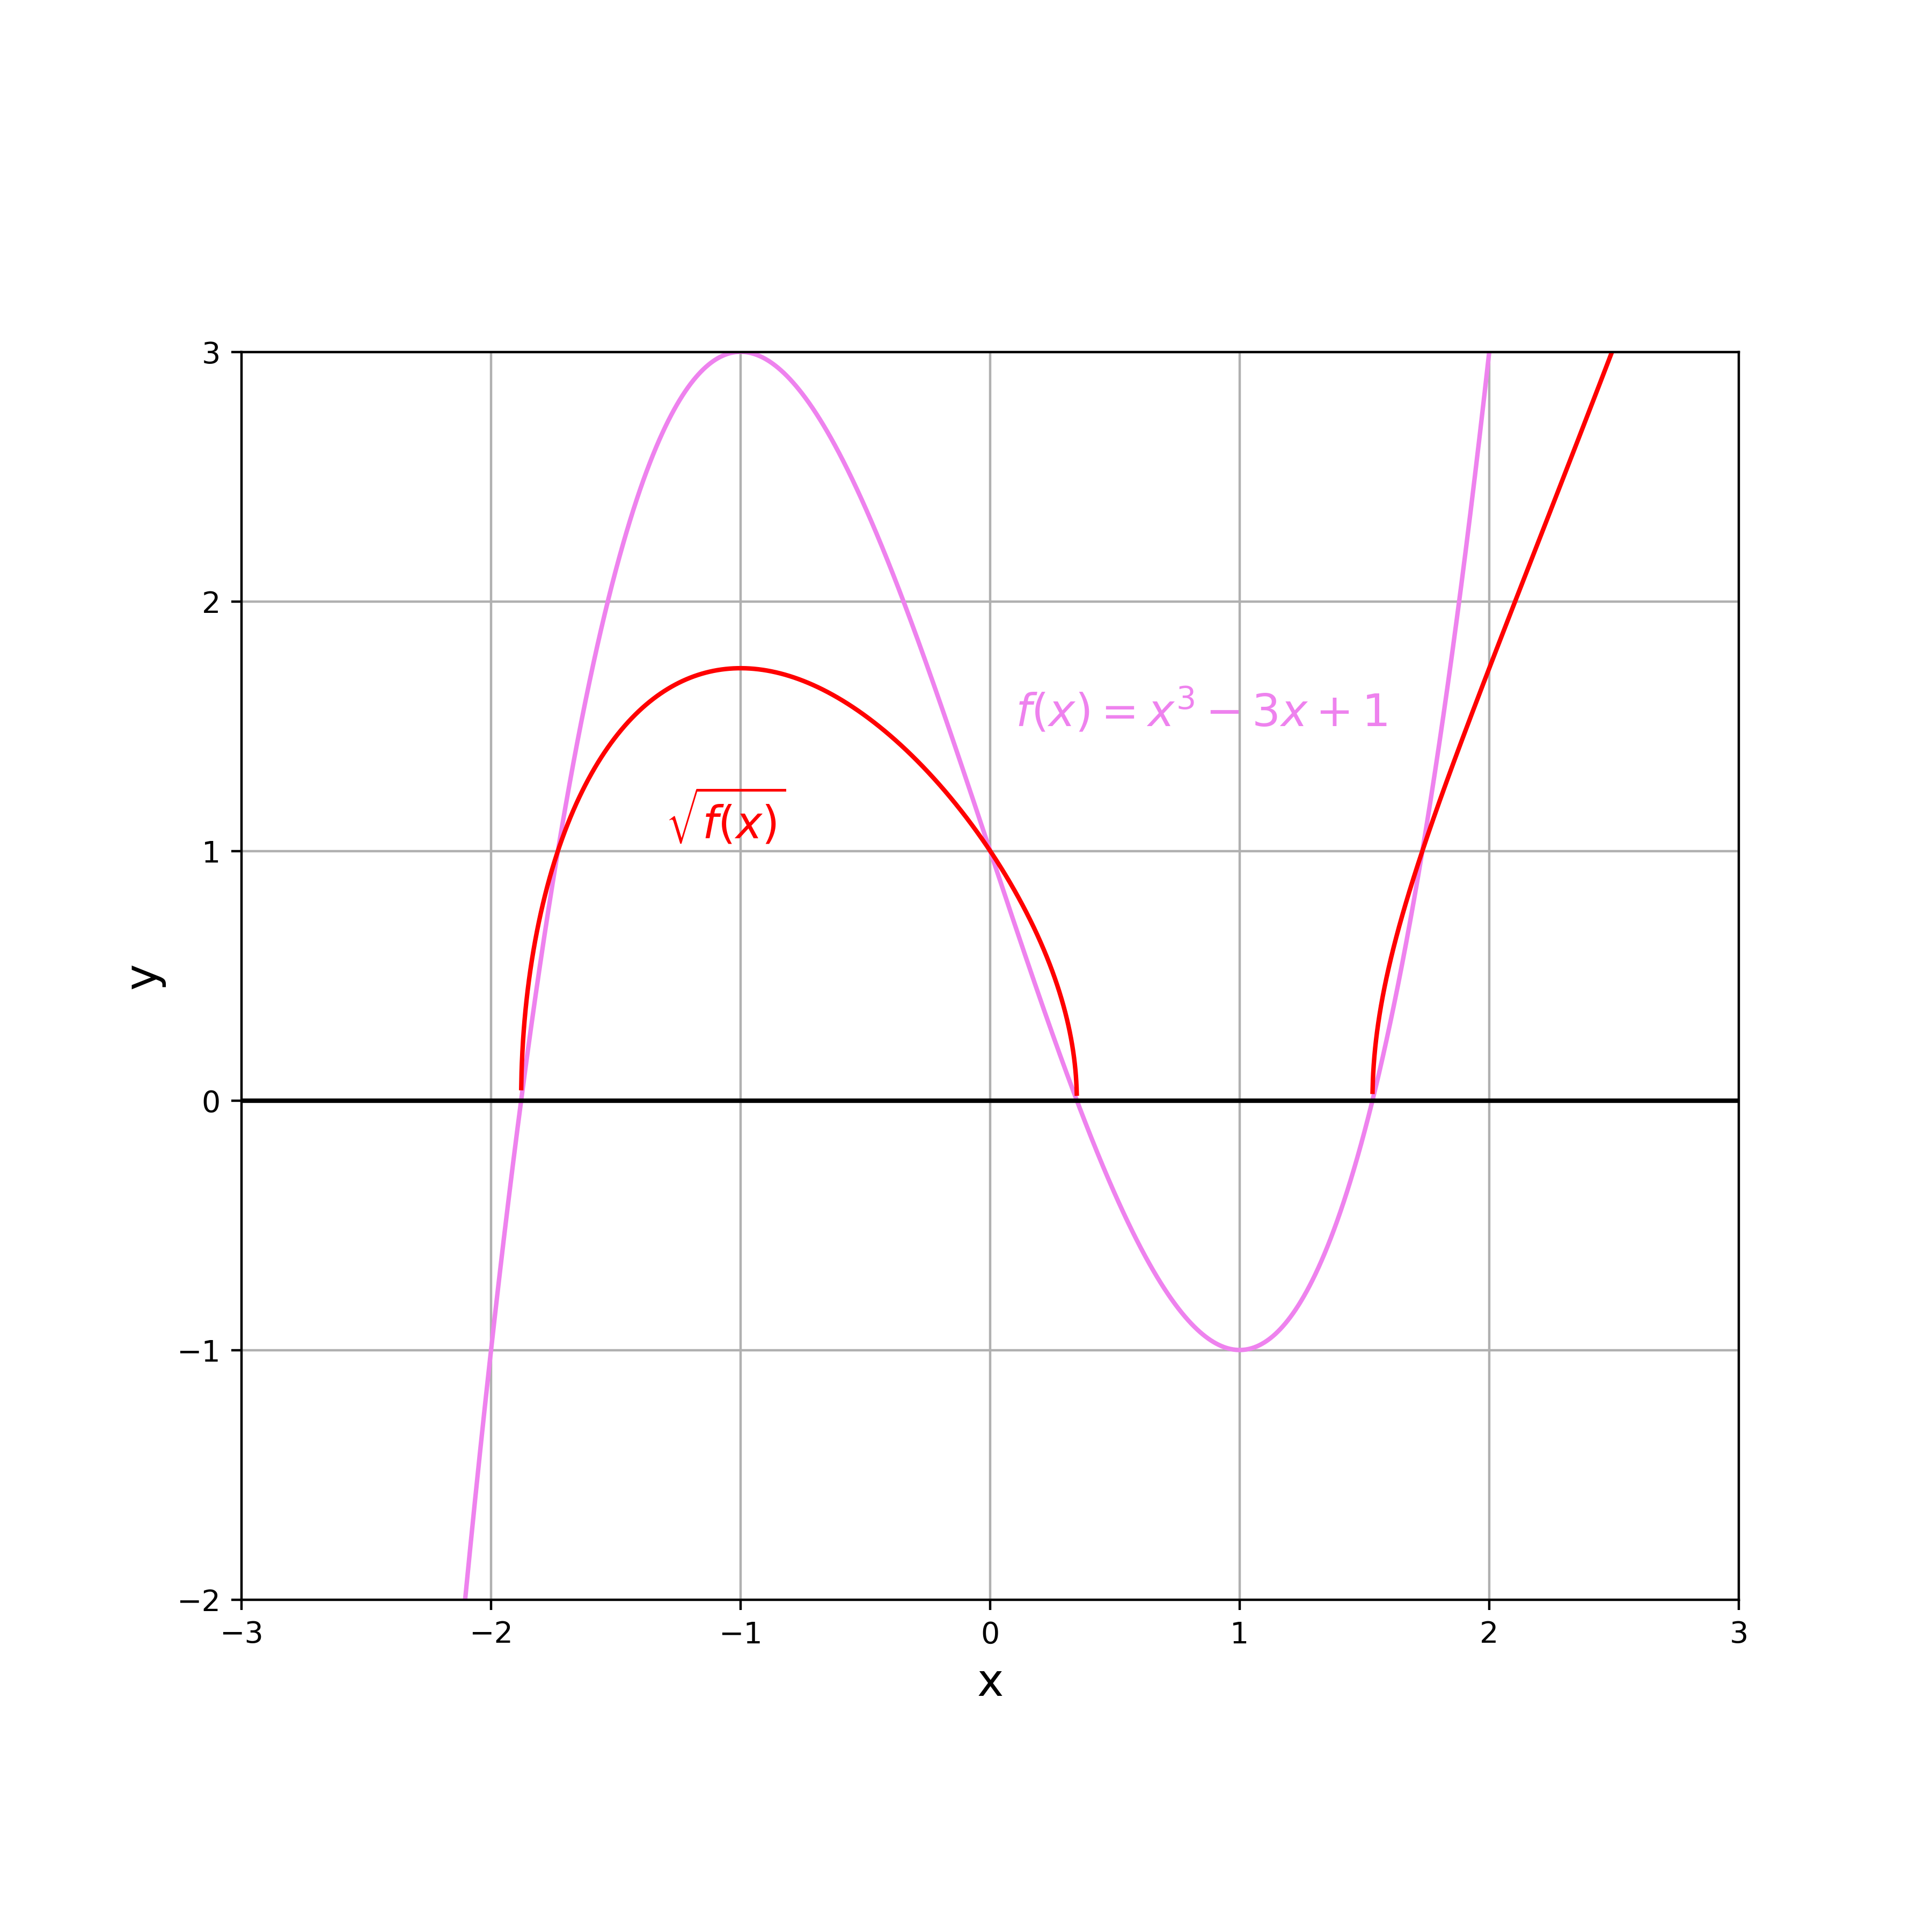
\includegraphics[width=\linewidth]{cubic_function.png} 
\caption{A depiction of how one branch of an elliptic curve arises from square-rooting a depressed cubic.}
\label{fig:cubicsqrt}
\end{center}
\end{figure}

\subsection{Geometric Secant-Tangent Construction}

It turns out, Elliptic curves are special because one can define a reasonable notion of addition with points on the curve. The one caveat is that we require a point 'at infinity' $I$ to do so. Formally, this means were working in the projective real plane $\mathbb{RP}^2$ or $\mathbb{R}^2 \cup \lbrace \infty \rbrace$. 
But with this, we obtain the property that any secant drawn through two points on the curve must intersect another third point on the curve or this point at infinity $I$. Thus we will define the addition of two points $P$ and $Q$ to be this third point reflected across the y-axis.\footnote{Note, without reflecting across the y-axis, this operation would not be associative. It also makes sense with the notion that three colinear points sum to the point-at-infinity $A+B+C=I$ and hence, $A+B=-C$.}

\begin{figure}[ht]
\begin{center}
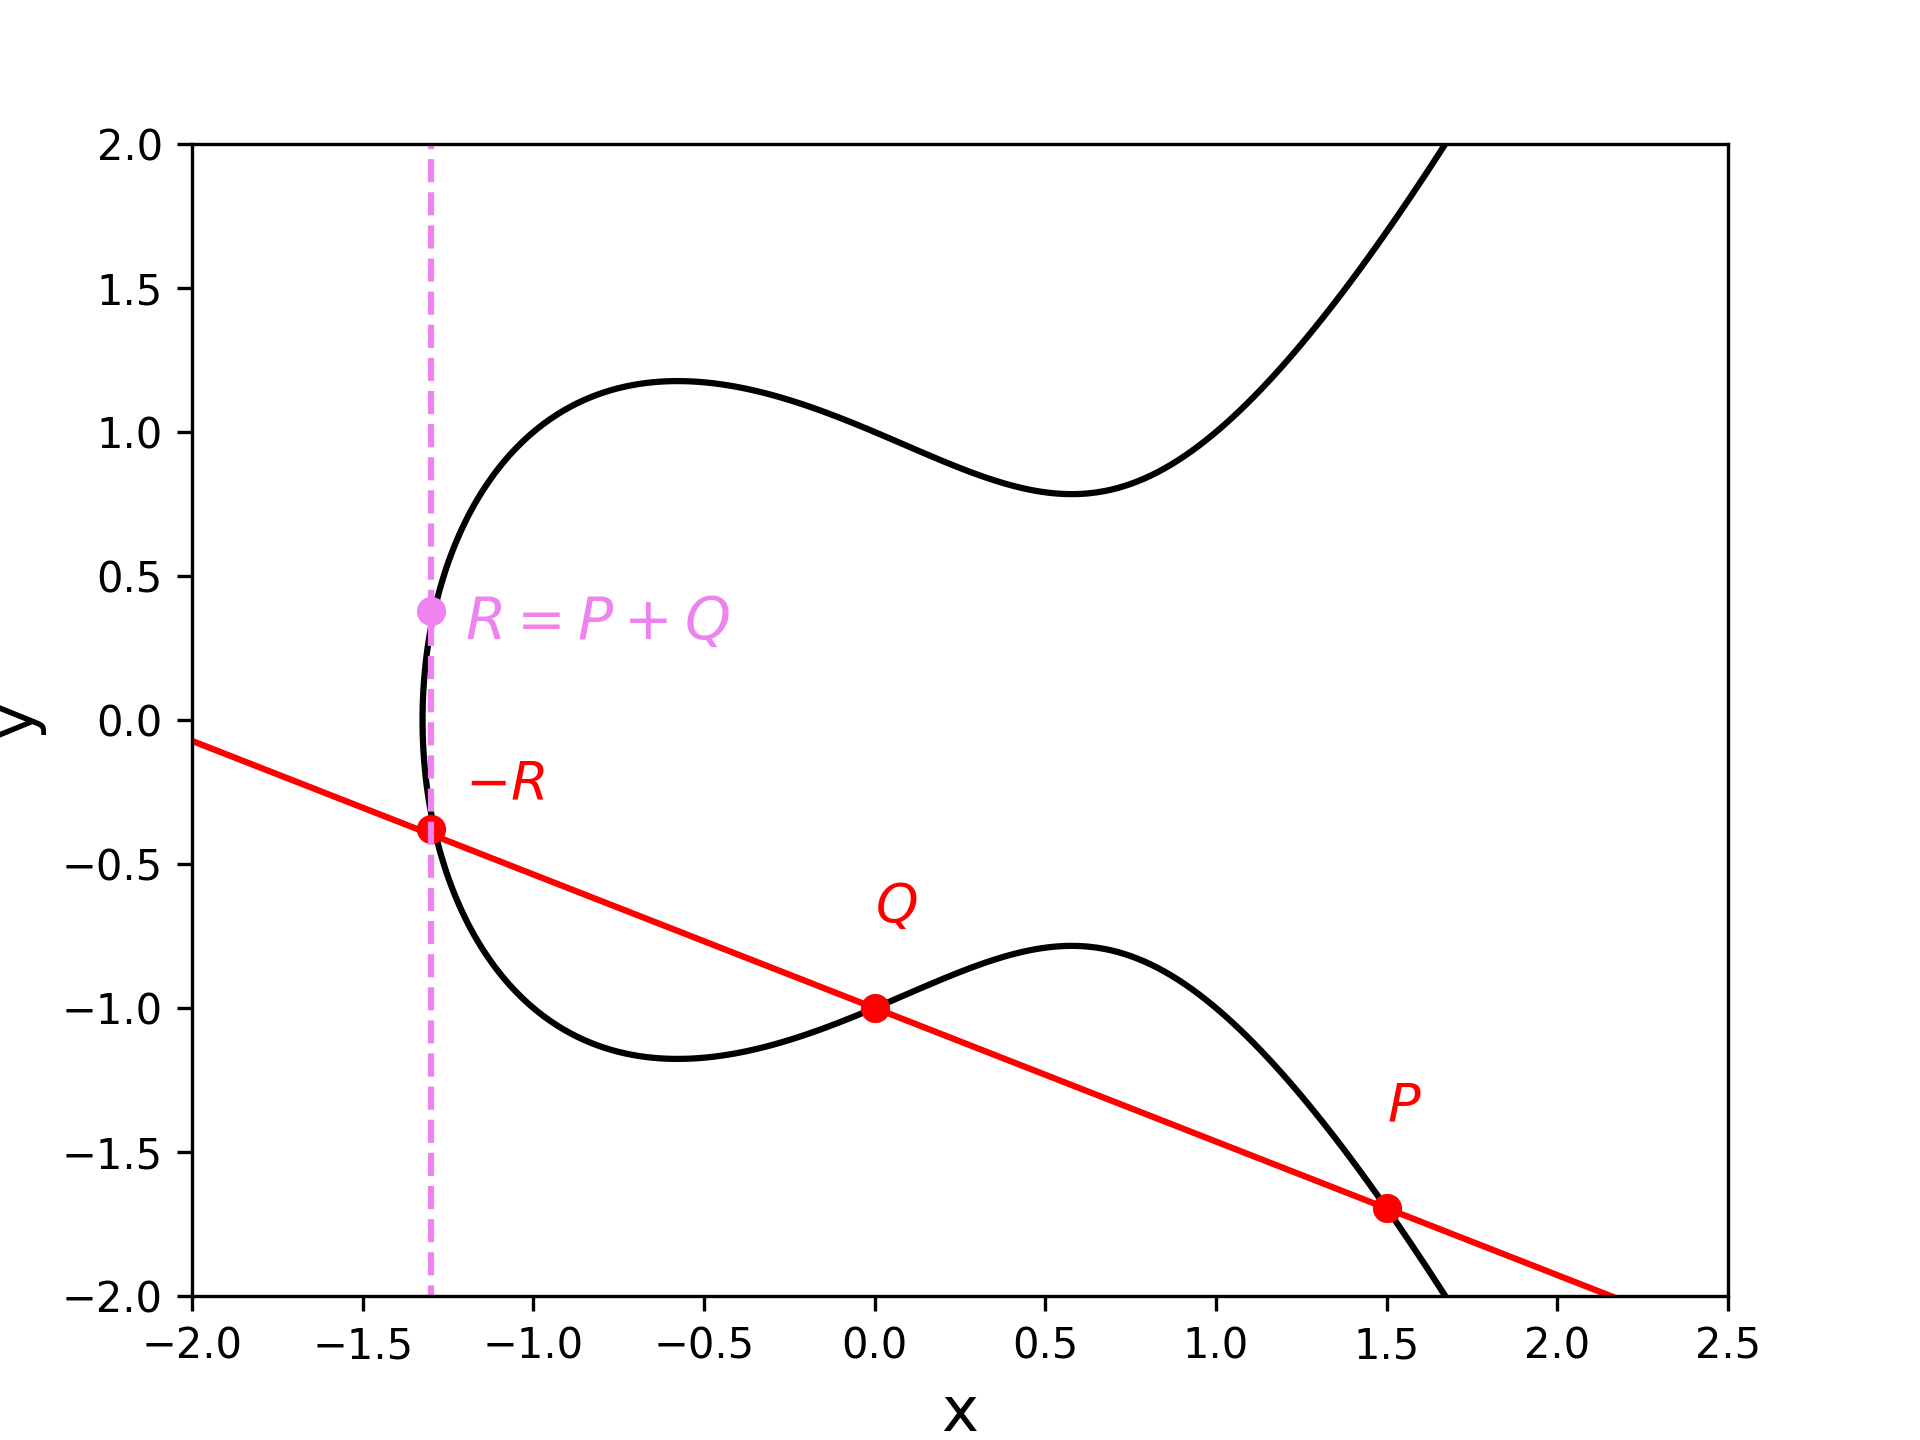
\includegraphics[width=\linewidth]{grouplaw.png} 
\caption{Point addition of two points $P$ and $Q$, defined by reflecting the third point of intersection across the y-axis, on $y^2 = x^3 -x+1$.}
\label{fig:additionEC}
\end{center}
\end{figure}

\subsection{Addition of Two Points}

We can make this idea rigorous by using some geometric tools. Our third point $-R$ is defined as the intersection of our elliptic curve $y^2 = x^3 + ax +b$ and some secant line $y=mx+l$. Given the points $P, Q = (x_p,y_p), (x_q,y_q)$ we can write down the slope:
\[m = \frac{y_p - y_q}{x_p-x_q}\]
Proceeding with the simultaneous equations
\begin{align}
y^2 &= x^3 + ax +b\\
y&=mx+l
\end{align}
Substituting (2) into (1),
\begin{flalign*}
(mx+l)^2 &= x^3 + ax +b\\
m^2x^2 + 2mlx + l^2 &= x^3 + ax +b \\
\Rightarrow 0 = x^3 - &(m^2)x - (2ml)x + (b-l^2) \tag 3
\end{flalign*}
Now, this cubic has three real solutions, namely the roots of P, Q and R respectively. Writing these as factors:
\[(x-x_p)(x-x_q)(x-x_r) = x^3 - (m^2)x^2 - (2ml)x + (b-l^2)\]
The next step is to expand the left side out and equate coefficients.
\begin{align*}
LH &= x^3 - \color{Purple}{(x_p+x_q+x_r)} \color{black}{x^2} +  (x_p x_q + x_px_r + x_qx_r) x  - x_px_qx_r\\
RH &= x^3\hspace*{1.6cm}  - \color{Purple}{(m^2)} \color{black}{x^2} \hspace*{2.4cm}  - (2ml) x  + (b-l^2). \text{\hspace*{1.2cm}}
\end{align*}
This means, using the purple coefficients,
\begin{align*}
m^2 &= x_p +x_q+x_r\\
\therefore \hspace*{0.3cm} x_r &= m^2 - x_p - x_q. \tag 4
\end{align*}
Substituting the x coordinate of $-R$, $x_r$ into the point-slope form of the line with $m = \frac{y_p - y_q}{x_p-x_q}$ we obtain,
\begin{align*}
y_r &= y_q + m(x_r-x_q)\\ 
&= y_p + m(x_r -x_p).
\end{align*}
Flipping our result across the y-axis to obtain $R$, we have (finally),\footnote{As long as $P \neq Q$ and $P \neq -Q$.}

\begin{align*}
P \; + \; Q \; &:= \; R\\
(x_p,y_p)+(x_q,y_q) &:= \left( m^2 -x_p-x_q,\;\  -y_q - m(x_r-x_q) \right),
\end{align*}
\begin{center}
where $m = \frac{y_p - y_q}{x_p-x_q}$.
\end{center}
\qed

\subsection{Inverse Points and Infinity}

In the case of adding two points opposite each other over the y-axis, one says they intersect the third point "at infinity." 
In general, over a projective plane, we revise the parallel postulate to say "any two parallel lines share one point of intersection, namely the point at infinity." We see this below; like train tracks meeting the horizon, the two parallel, vertical lines meet at $\infty$ or $I$. 

\begin{figure}[ht]
\begin{center}
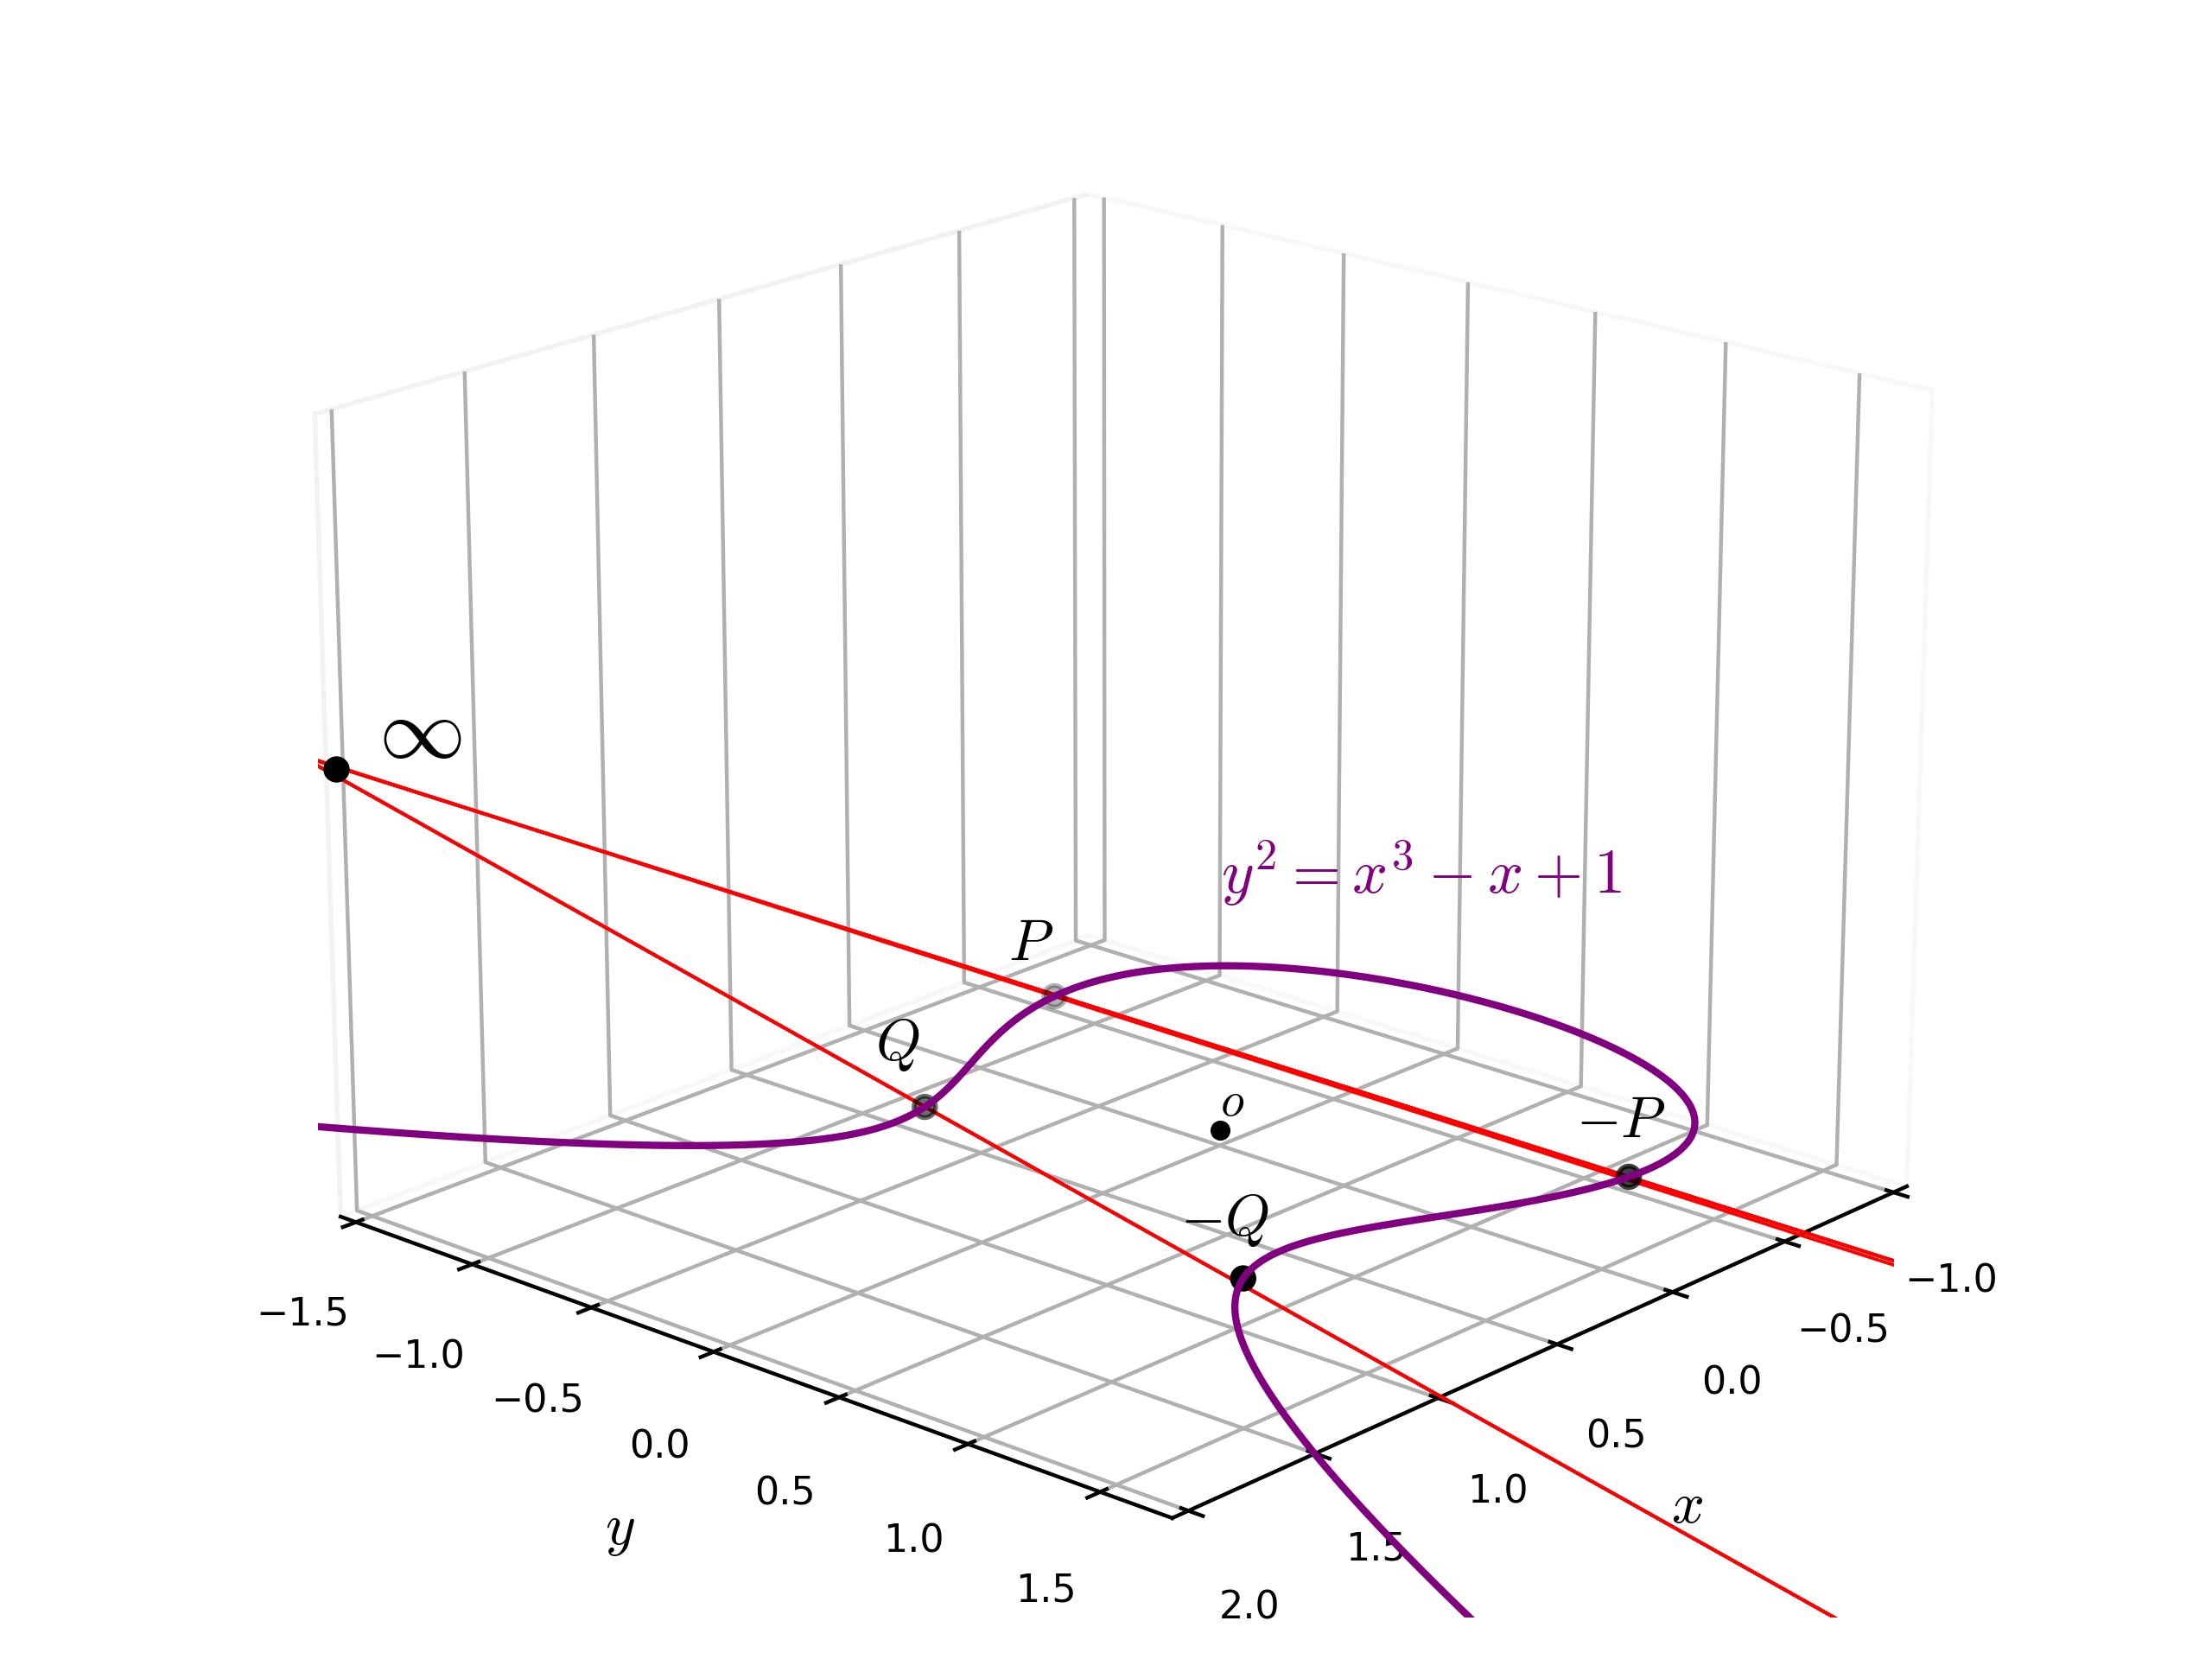
\includegraphics[width=\linewidth]{3dplot.png} 
\caption{Parallel lines drawn through inverse points, all intersecting at point at infinity $I$ over $y^2=x^3 - x + 1$. As in, $P + (-P) = I = Q + (-Q)$.}
\label{fig:3dproj}
\end{center}
\end{figure}

Because of this construction, $I$ acts as a left- and right-sided identity element. Since, for any ($\reals$-rational) point $A$ with inverse $-A$ on the elliptic-curve,
\begin{align*}
  A + (-A) &= I\\
  A + (-A)\; \color{blue}{+ A} &= I \color{blue}{+ A}\\
  \Rightarrow \hspace*{0.3cm} A + I &= I + A = A \tag 5
\end{align*}


\subsection{Adding a Point to Itself}
The case that was left out of the earlier pictorial representation of point addition is when a point is added to itself. Not to fear, however, since we can replace the secant through two points with a tangent through one. The resultant point is the resultant intersection flipped across the y-axis. The slope of this tangent can be found through implicit differentiation.
\begin{align*}
\color{red}{d(}\color{black}{y^2}\color{red}{)} &= \color{red}{d(}\color{black}{x^3+ax+b}\color{red}{)}\\
2y\color{red}{dy} &= 3x^2\color{red}{dx} \color{black}\; { + \; a} \color{red}{dx}\\
\color{red}{\frac{dy}{dx}} &= \frac{3x^2 + a}{2y}.
\end{align*}
Thus with,
\[y_r-y_p = m(x_r-x_p)\]
\begin{center}
where $m = \frac{3x_p^2+a}{2y_p}$,
\end{center}
we can use the same result as before with $P=Q$:
\begin{align*}
m^2 &= x_p +x_q +x_r\\
\Rightarrow \hspace*{0.3cm} x_r &= m^2 - 2x_p \tag 6\\
\end{align*}
and, using the point-slope form and flipping across the y-axis, 
\begin{align*}
y_r = -y_p-m(x_r-x_p)
\end{align*}
\qed

*A word on notation: the choice to use $+$ to denote this binary operation is entirely arbitrary, and many authors use alternate notation to represent this ($\times, \oplus,\otimes,\star$ etc.). Using $+$ hints that adding a point $P$ to itself $n$ times might be written $nP$, but for sake of consistency with the theory to come, I will write this $P^n$ meaning $P+P+...+P$, $n$-times. This will make sense in a moment.

\section{Group structure of $E[K]$}

\subsection{Verifying the Group Axioms}

By the higher powers of mathematical serendipity, this forms a group! A very special group at that. We can write this elliptic curve group as $E[\reals]$ for the case in the reals. Or, $E[K]$ for any field $K$ (again, a structure with $+, -, \times, \div$).

	Now, we will (at least, heuristically) verify that the group axioms hold, we first see in eq (5) that we have a two-sided identity, $I$, given by the point at infinity. Hence,
\[ P + I = I + P = I \; \text{ for all } P \in E[K] \]
Next, we prove the existence of an inverse for every element by noticing that our curve is symmetric about the y-axis. Similarly our identity element $I$ is self-inverse. Hence,
\[ \text{for all } P \in E[K], \text{ there exists an inverse } -P \text{ such that } P + (-P) = I \]
This operation is associative as well, but unfortunately a rigorous proof of this fact is unprecedentedly untame, especially through this geometric depiction of elliptic curves. With more powerful tools from algebraic geometry, this proof is almost trivial, following nicely from  tracking values on points of a curve (namely $\mathrm{Div}^0(E)$) and the relationship between poles and zeros, as stated by the Riemann-Roch theorem.\autocite[66]{silverman}
Lastly, this binary operation of adding two points is \textit{commutative} as well, following geometrically from the secant construction or through the formulas.

As a result of meeting these conditions, $E[K]$ forms an abelian group under our binary operation.

\subsection{Finite Fields $\field_p$}

This elliptic curve group action holds for other fields $K$ as well. Most important to cryptography is elliptic curves over "finite" fields. 
A finite field, denoted $\field_p$ for $p$ prime,\footnote{Technically, $p$ can be a prime power. 
One might write $\field_q$ where $q = p^r$.} is a set of ordered pairs $(x,y)$ with addition, subtraction and multiplication taken \textit{modulo $p$}. 

As I alluded to earlier, the condition that $p$ be prime is so that every element $n < p$ has a multiplicative inverse, since, to have a multiplicative inverse, $\mathrm{gcd}(n,p)=1$. Really, finite fields are the elements of $\integers / p \integers$ with addition and multiplication in $(\integers / p \integers)^{+}$ and $(\integers / p \integers)^{\times}$. The field axioms readily follow from the group axioms of the multiplicative and additive groups.

\subsection{Elliptic Curves over Finite Fields, $K = \field_p$}

Using the same equations from before, except with operations taken \textit{modulo} $p$, this elliptic curve still forms a group over a finite field, $E[\field_p]$. The elements of this group are the points, 
\[ E[\field_p] = \left\lbrace (x,y)\ |\ y^2 \equiv x^3 + ax + b \bmod p \right\rbrace \cup \lbrace \infty \rbrace. \]
with the additional $\infty$ element serving as the identity.

Plotting examples of these groups over finite fields, we see the geometric intuition breaks down somewhat.
\begin{figure}[ht]
\centering
\begin{subfigure}{0.49\textwidth}
\centering
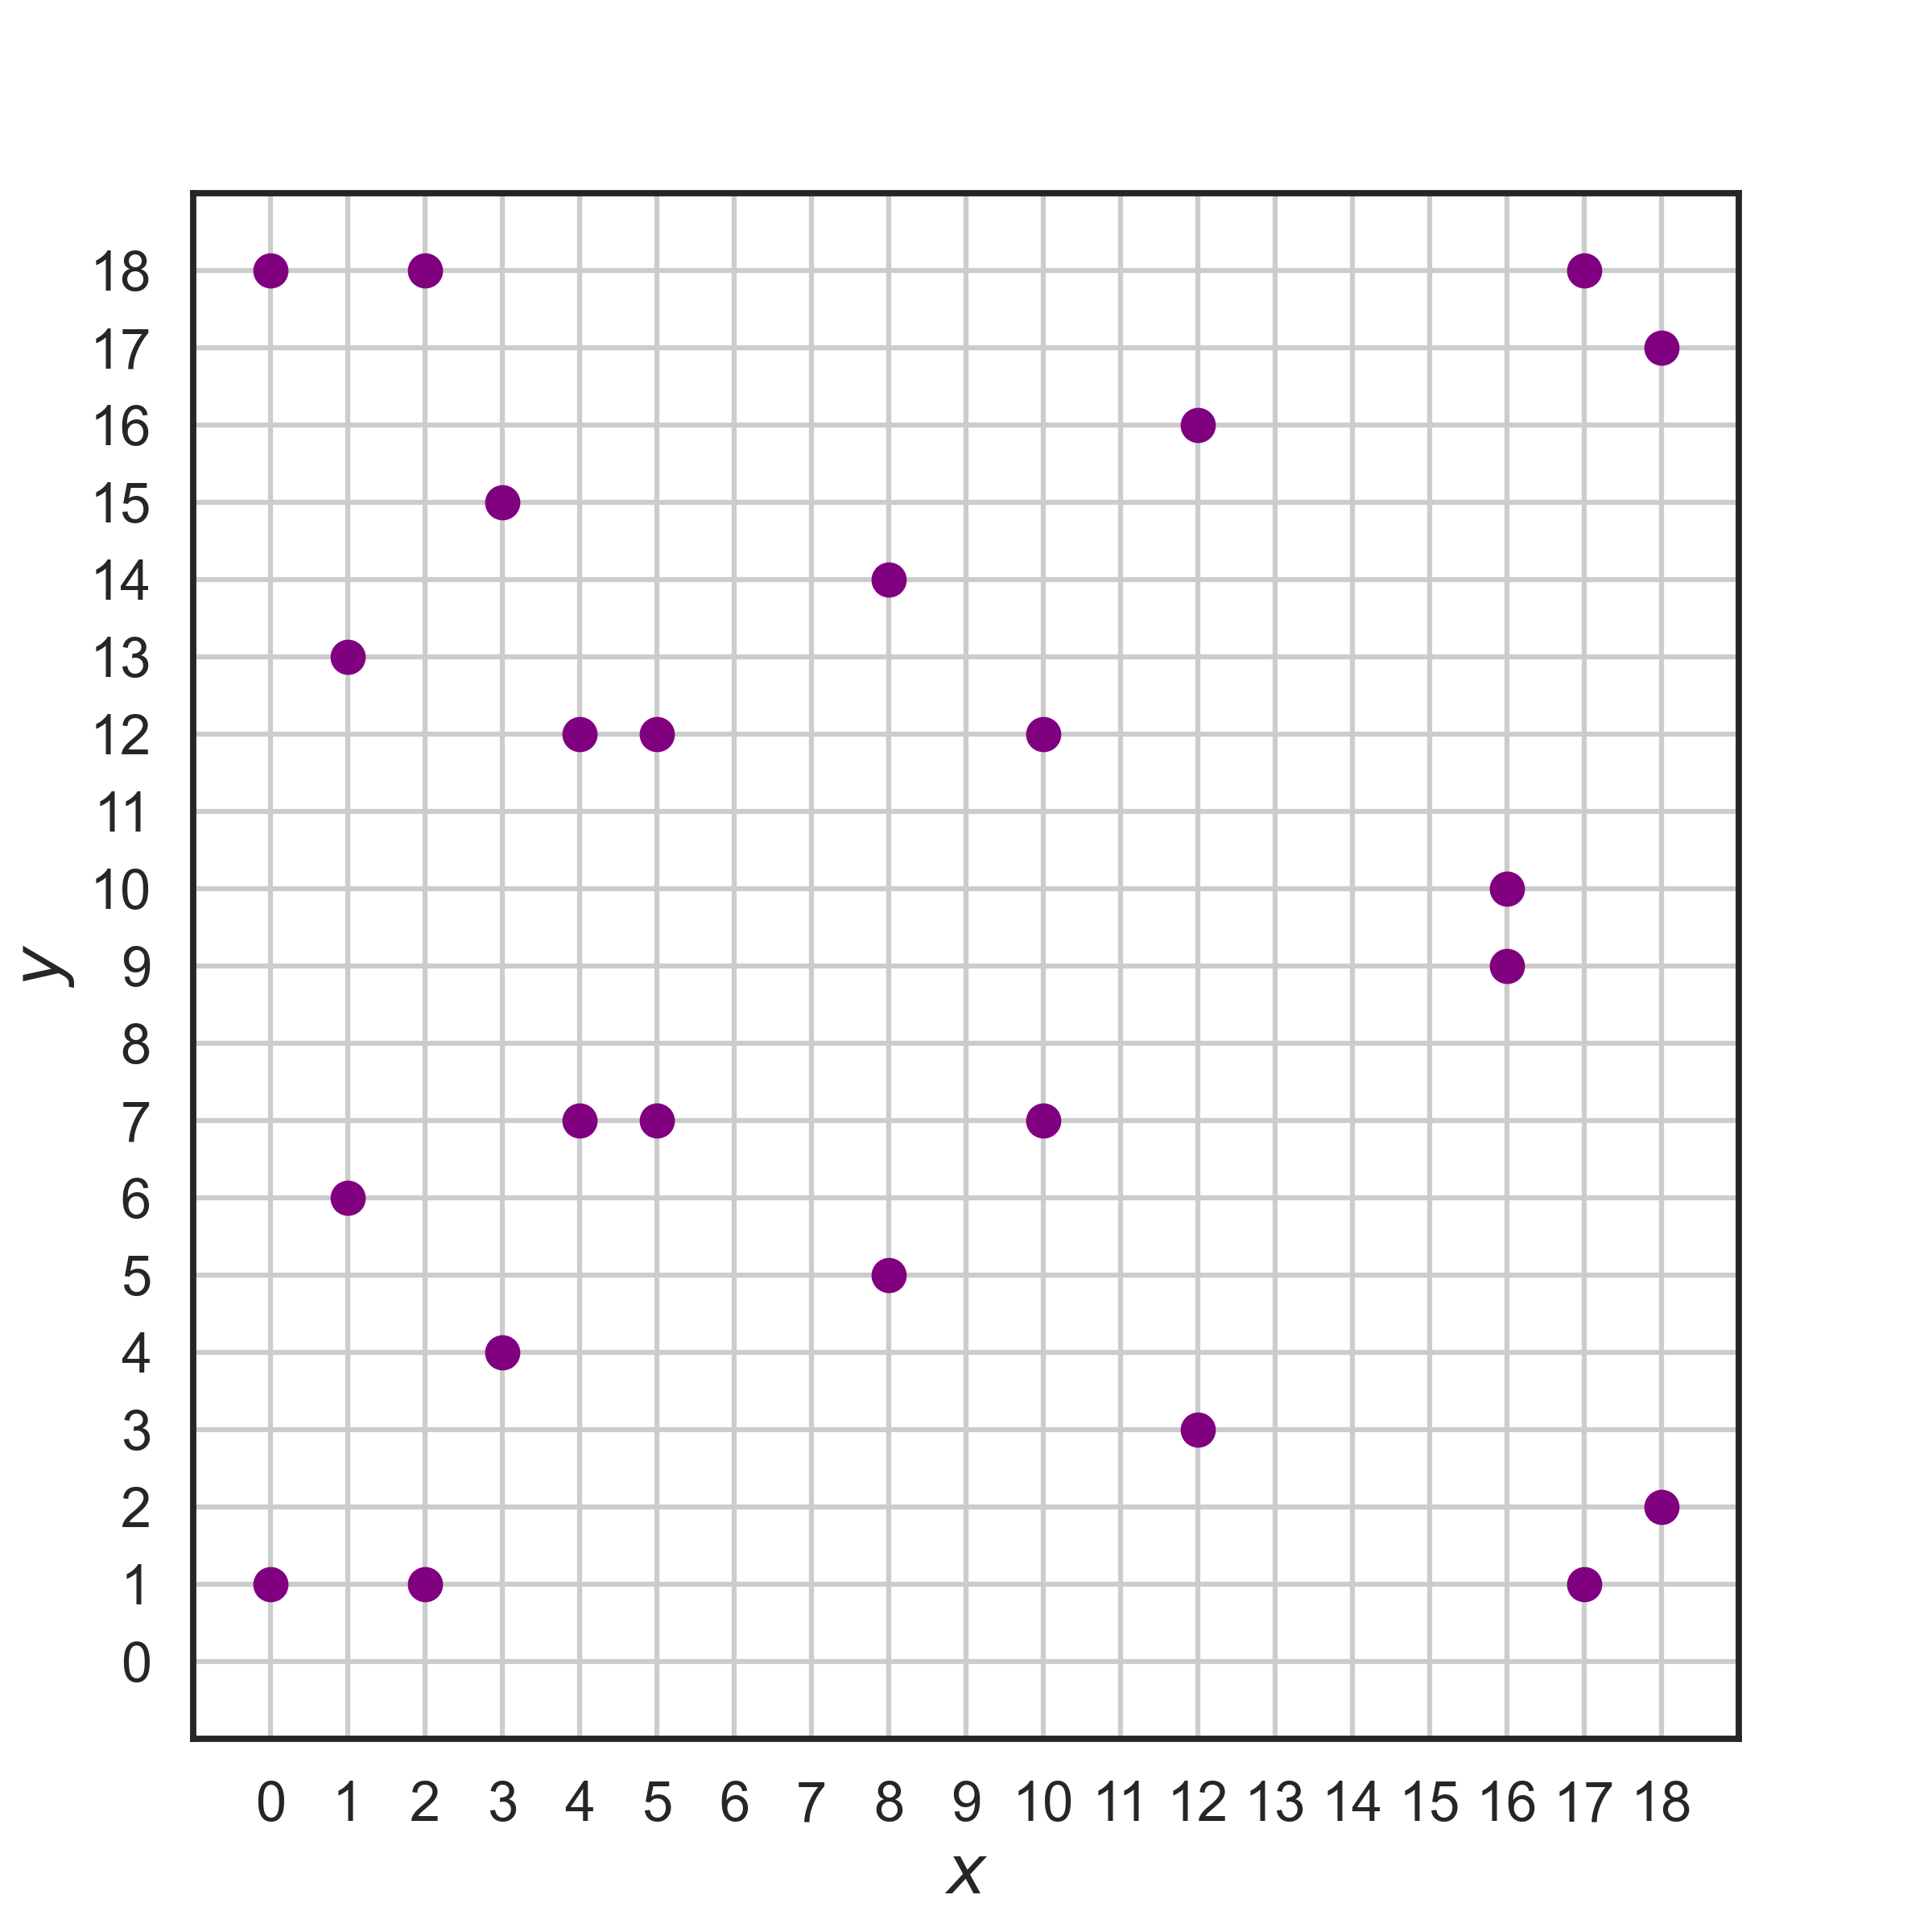
\includegraphics[width = \textwidth]{krationalpoints19.png}
\caption{$y^2 = x^3 + 15x + 1$ over $\field_{19}$}
\label{fig:left}
\end{subfigure}
\begin{subfigure}{0.49\textwidth}
\centering
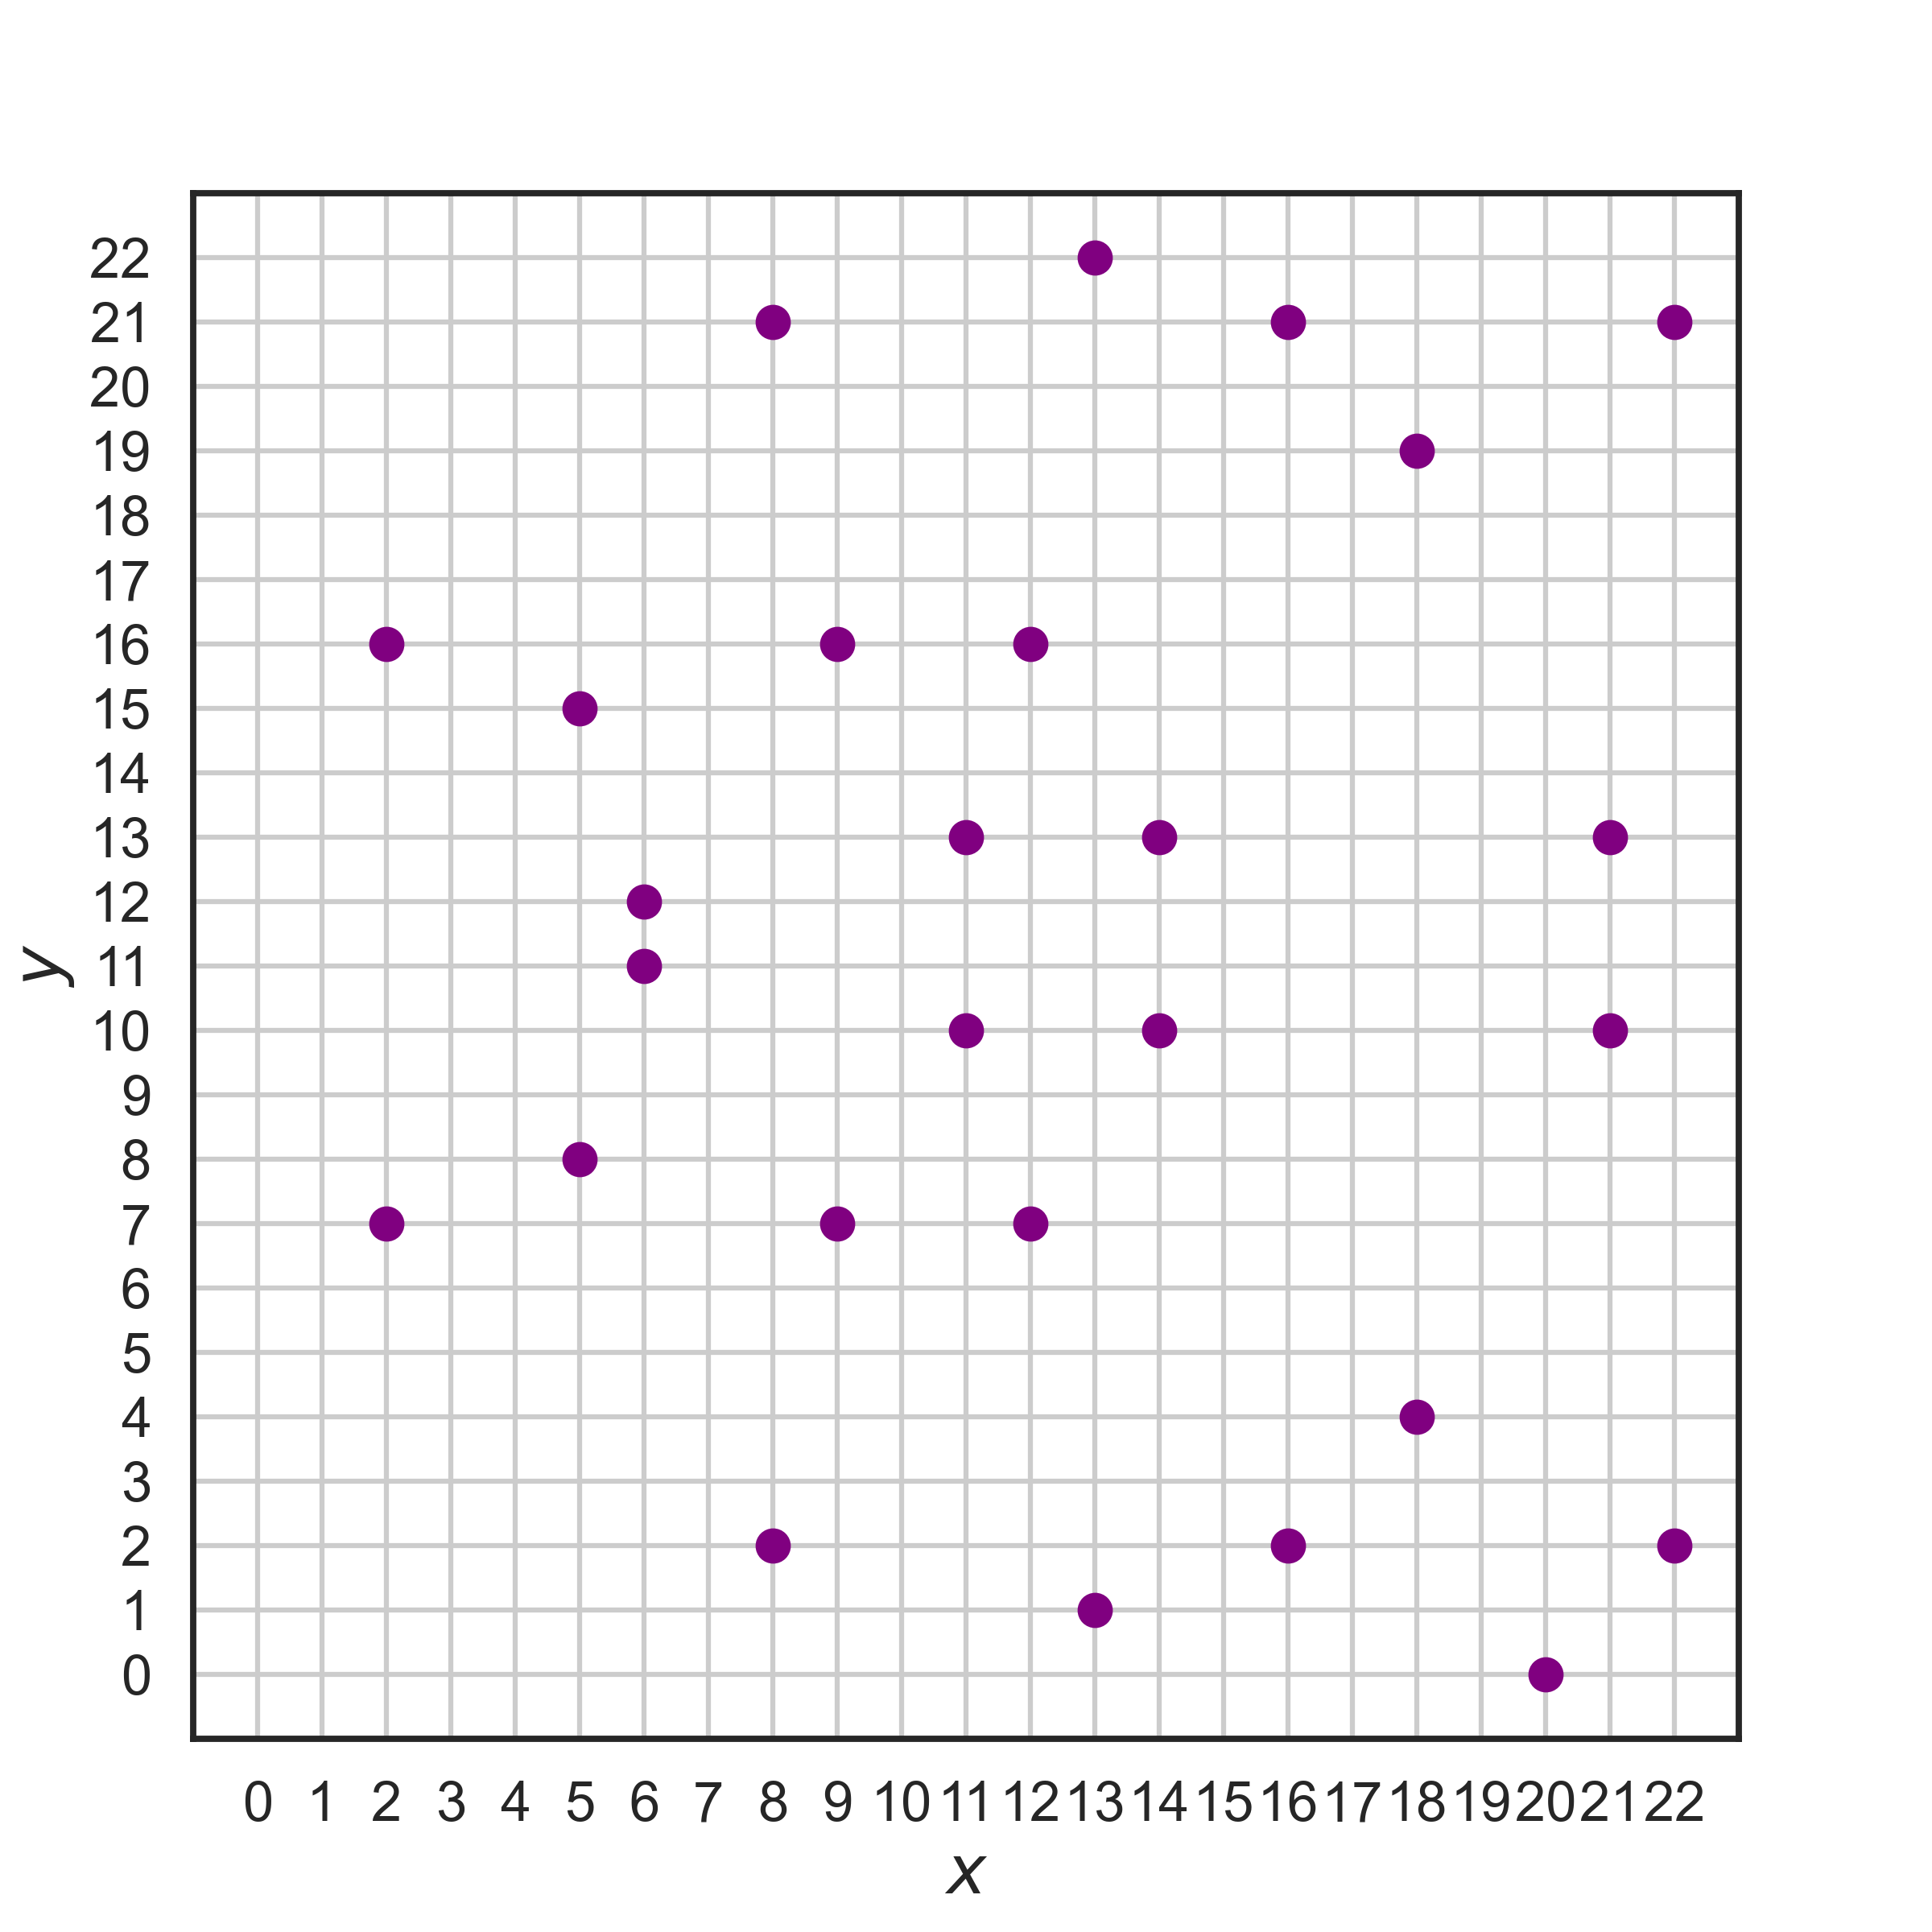
\includegraphics[width = \textwidth]{krationalpoints23.png}
\caption{$y^2 = x^3 + 12x + 17$ over $\field_{23}$}
\label{fig:right}
\end{subfigure}
\caption{Select elliptic curves plotted over finite fields. Notice the symmetry about $\frac{p}{2}$.}
\label{fig:combined}
\end{figure}

In an attempt to better understand the group structure, I coded an interactive web-app in Typescript that computes the multiplication table of the group elements, known as a Cayley table. The symmetry about the diagonal indicates the commutativity as well.

\begin{figure}[ht]
\begin{center}
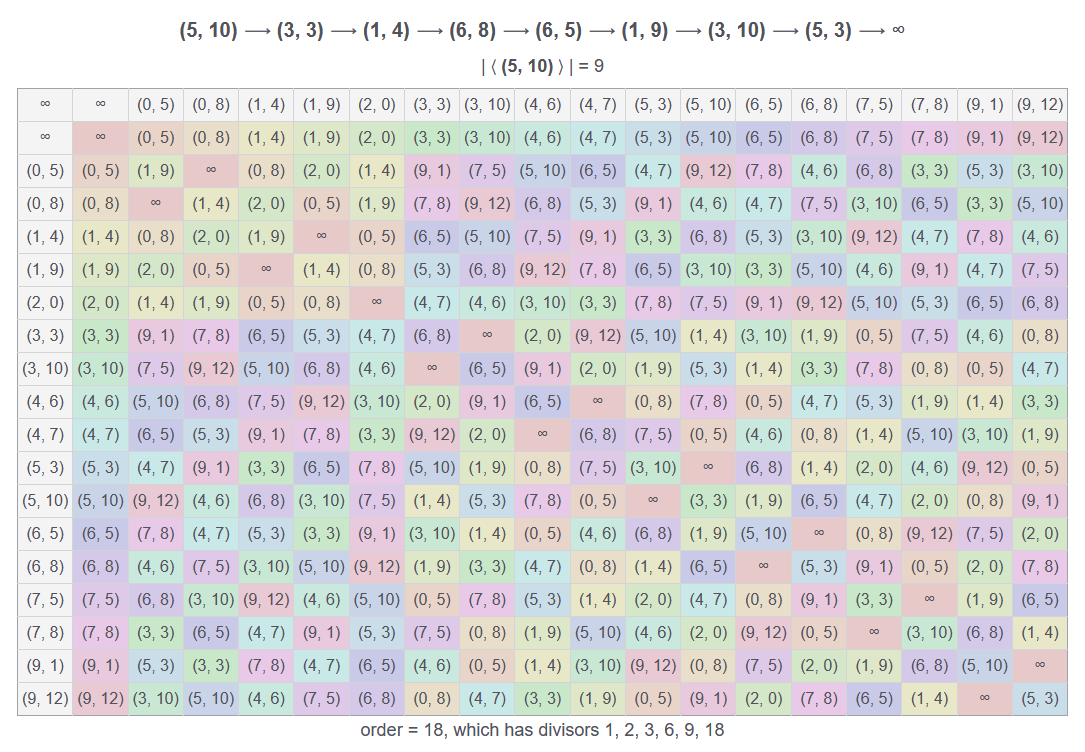
\includegraphics[width=\linewidth]{cayleytable.png} 
\caption{App on my \href{jacobbruner.com/elliptic-curve}{personal website} computing the Cayley table of $y^2 = x^3 + 3x + 12$ over $\field_{17}$. Clicking on an element computes the subgroup it generates, the focused point being $(5,10)$ here.}
\label{fig:cayley}
\end{center}
\end{figure}

Using the elements of this elliptic curve group, one can formulate a new form of Diffie-Hellman key exchange where, given a suitable generator point $g$, all the repeated multiplications can be performed on this elliptic curve group. The benefit of doing this is that the structure of an elliptic curve group $E[\field_p]$ is much more complicated than that of $(\integers / q \integers)^{\times}$. When working in $(\integers / q \integers)^{\times}$, there are number-theoretical properties making it easier to narrow down guesses, especially when computing a discrete logarithm problem as discussed earlier. Diem, C. (2011) showed that that the discrete logarithm problem for elliptic curves has an asymptotic time complexity greater than that of $(\integers / q \integers)^{\times}$.\autocite[76]{diem} The culmination of this research into elliptic curve cryptography is the fact that most public key protocols utilize elliptic curves in one way or another. 

\iffalse
\begin{figure}[ht]
\begin{center}
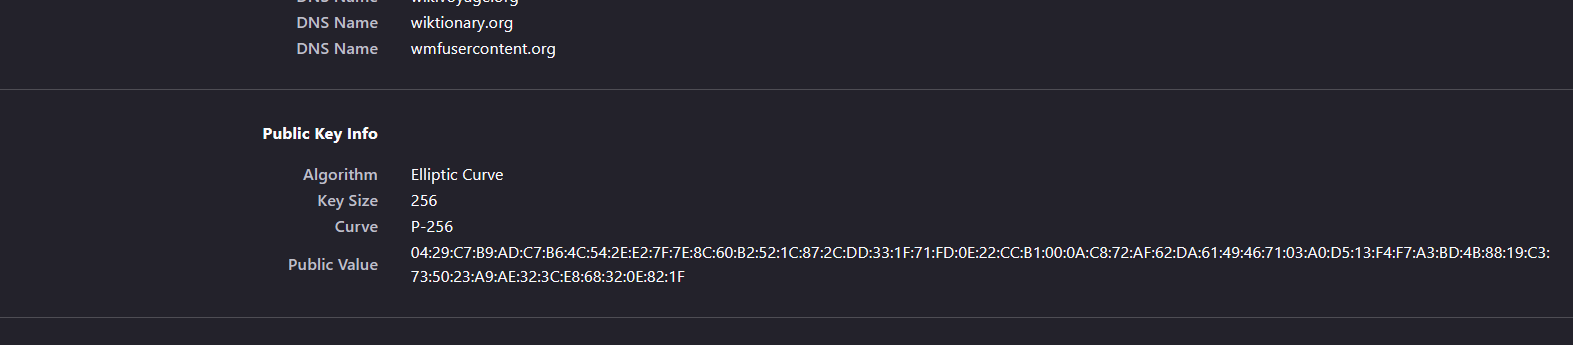
\includegraphics[width=\linewidth]{wikicert.png} 
\caption{Certificate information for wikipedia showing the use of elliptic curve cryptography.}
\label{fig:wiki}
\end{center}
\end{figure}
\fi

\section{Conclusion}

In this paper, I sought to explore \textbf{to what extent does group theory provide a mathematical backdrop for modern public-key cryptography?} Resulting from my findings, it is clear that group theory does indeed provide a rich backdrop for discussing cryptographic concepts. Especially as computing power grows cheaper, the use of group-theoretical techniques to strengthen existing principles is paramount. For instance, the Diffie-Hellman protocol works on any abelian group. Further research is underway at examining other candidates for 'secure' groups, such as the study of hyperelliptic curves and other higher-genus abelian varieties (a variety forming an abelian group).

In the process of researching, it's clear that there are two different mathematical perspectives introducing elliptic curves. The decision was made to continue with the simpler route, defining the elliptic curve as the solution to a polynomial equation. However, this is not strictly necessary, since elliptic curves arise in many other contexts, like through the intersection of two quadric surfaces (like a 3-sphere and a hyperboloid for instance). The other route is a more theoretical perspective, using tools from algebraic geometry and topology to reach the same conclusions as the simpler route. The benefit of approaching it this way, however, is that these tools can be generalized to other contexts to discover new group-theoretical perspectives on cryptography. Doing so also would decrease the 'arbitrary-ness' of some of the topics explored in this paper. Coming at a topic from the top-down can make certain difficult proofs and perspectives trivial, as I mention a couple times in the paper.

Another aspect of this paper worth mentioning is the impercise handling of comparison between elliptic curve cryptography and traditional cryptography. Going into it, I intended to explore the nitty-gritty details of the elliptic curve group structure, detailing exactly why the hidden-subgroup problem and discrete logarithm problem were more difficult. This proved to be much more challenging than I anticipated, and, although I satisfied some of my own curiosity in researching, I knew it would be an impractical undertaking to convey the wealth of prerequisites in this paper to reach the conclusions I wanted. As a result, my research question lacks some of the 'argument' I wanted it to have, rather opting for a more expository lens on this complicated subject. Regardless, I find this is a subject that is fruitful to learn because of it's reasonable ties to number theory and its underappreciated influence on modern-day life.


\newpage 

\printbibliography

\end{document}
